\documentclass[12pt]{article}
% We can write notes using the percent symbol!
% The first line above is to announce we are beginning a document, an article in this case, and we want the default font size to be 12pt
\usepackage[utf8]{inputenc}
\usepackage[left=1.2in,top=.8in,right=1.2in,nohead,bottom=.5in]{geometry}
% This is a package to accept utf8 input.  I normally do not use it in my documents, but it was here by default in Overleaf.

\usepackage{amssymb}
\usepackage{amsthm}
\usepackage{commath}
\usepackage{enumerate}
\newtheorem{theorem}{Theorem}
\usepackage{amsmath}
\usepackage{natbib}
\usepackage{graphicx}
\usepackage{caption}
\usepackage{subcaption}
\graphicspath{ {./plots/} }
\DeclareMathOperator{\Tr}{Tr}
\newcommand{\dd}[1]{\mathrm{d}#1}
\newcommand{\E}{\mathbb{E}}
\newcommand{\Var}{\text{Var}}
\newcommand{\X}{\mathcal{X}}
\newcommand{\B}{\mathcal{B}}
% These three packages are from the American Mathematical Society and includes all of the important symbols and operations 
\usepackage{fullpage}
\usepackage{comment}
% By default, an article has some vary large margins to fit the smaller page format.  This allows us to use more standard margins.

\newtheorem{ass}{Assumption}
\newtheorem{lemma}{Lemma}
\newtheorem{corollary}{Corollary}
\newtheorem{remark}{Remark}
\setlength{\parskip}{0em}
% This gives us a full line break when we write a new paragraph
\usepackage[mathscr]{euscript}
\usepackage{tikz}
\newcommand*\circled[1]{\tikz[baseline=(char.base)]{
            \node[shape=circle,draw,inner sep=2pt] (char) {#1};}}
\newcommand{\indep}{\perp \!\!\! \perp}
\title{Estimating autocorrelation from multiple Markov chains}

\author{
  Medha Agarwal \\
  \textit{Department of Mathematics and Statistics}\\
  \textit{IIT Kanpur}\\
  \texttt{medhaaga@iitk.ac.in} \\\\
  %% examples of more authors
 Dootika Vats \\
  \textit{Department of Mathematics and Statistics}\\
  \textit{IIT Kanpur}\\
  \texttt{dootika@iitk.ac.in} \\
}


\begin{document}

\maketitle


\begin{abstract}
    This is best abstract in the world.\\.\\.\\.\\.\\.
\end{abstract}


\section{Introduction} \label{sec:intro}

Markov chain Monte Carlo (MCMC) is a sampling method used to obtain correlated realizations from a stochastic process. Due to this serial correlation in observations, a large number of MCMC samples are required to estimate features of the target distribution as compared to the independent ones. Therefore, it becomes imperative for an MCMC practitioner to have an idea about underlying dependence structure in the Markov chains. Autocovariance function (ACF) characterizes this dependence for a stationary Markov chain. A famous sample autovariance function is the empirical estimator, which unfortunately comes with its drawbacks. Firstly, it is not immune to outliers (see \cite{ma2000highly}) and secondly, it is usually non-informative in case of slowly mixing Markov chains for decently finite samples. We address the second issue in this paper by using multiple representative samples of the target distribution via parallel Markov chains.\\

Calculation of exact theoretical ACF has been done for simple models like autoregressive (AR), moving average (MA) (\cite{quenouille1947notes}), and autoregressive-moving-average (ARMA) (\cite{box2015time}) models. However, for most of the complex processes, we rely on sample ACF to understand the correlation in the chain at a particular lag. For a slowly mixing Markov chain or a multi-modal target distribution, Markov chains explore the sample space only partially for even high sample size. In such situations, single chain empirical ACF will underestimate the autocovariance giving misleading inferences. With convenient multi-core computation resources, it is possible to get multiple Markov chains for a target distribution.  We propose a new autocovariance estimator called replicated autocovariance function (R-ACF) with a simple fix in centering a chain about the overall mean. An important application of ACF is in calculating the asymptotic variance in the CLT of a Markov chain process.   \\

Suppose $F$ is the target distribution on support $\chi \subseteq \mathbb{R}^d$. For $g:\chi \longrightarrow \mathbb{R}^p$ be an F-integrable function. We are interested in

\[
\mu_g = \mathbb{E}_F[g(X)] = \int_{\chi}g(x)F(dx)
\]

Suppose we have $m$ replications of Markov chains with $n$ samples in each chain. Let $\{X_{st}\}_{t \geq 1}$ denote the $s^{th}$ Harris ergodic (aperiodic, F-irreducible, and positive Harris recurrent) Markov chain having invariant distribution $F$. We will use the following Monte Carlo estimator in order to estimate $\mu$ for the $s^{th}$ chain

\[
\hat{\mu}_s = \dfrac{1}{n}\sum_{i = 1}^{n} g(X_{si}) \xrightarrow{a.s.} \mu \textrm{ as } n \to \infty
\]

Throughout this paper, we will deal with the function $g(X) = X$. We denote the sample mean of $s^{th}$ Markov chain by $\overline{X}_s$ and the overall mean by $\overline{\overline{X}} = \sum_{s = 1}^{m}\overline{X}_s/m$. We are interested in Monte Carlo error, i.e. $\overline{\overline{X}} - \mu$ to assess the reliability of simulations. The sampling distribution for Monte Carlo error of $s^{th}$ chain is available via Markov chain CLT (\cite{jones2004markov}) if there exists a positive definite matrix $\Sigma$ such that

\[
\sqrt{n}(\overline{X}_s-\mu) \xrightarrow{d} N(0,\Sigma)
\]

 With $m$ i.i.d. samples of $\overline{X}_s$, $s \in \{1,..., m\}$, the MCSE is given by $\Sigma/mn$. We are interested in consistent estimates of $\Sigma$ for two reasons. Firstly, to construct asymptotically valid confidence intervals and secondly, to determine when to stop the simulations. For this purpose, we use the class of Multivariate Spectral Variance Estimators (MSVE) wherein we use R-ACF to estimate the autocovariance. We call this replicated spectral variance (RSV) estimator (see \cite{arg:and:2006} for replicated batch means). \\
 
MCMC ensures asymptotic convergence, however this is not practically very useful where the number of samples is finite. There are many criteria for terminating simulation like fixed-time rule, sequencial fixed-volume rule (see \cite{glynn1992asymptotic}), and using Gelman Rubin diagnostics (\cite{gelman1992inference}). The relative fixed-volume rule has been thoroughly discussed for MCMC by \cite{flegal2015relative} and \cite{gong2016practical}. We will use method of effective sample size (ESS) defined by \cite{vats2019multivariate} for terminating the simulations. The quality of estimation of $\Sigma$ is critical in determining that the simulations are not stopped prematurely. \\
 
Markov chains are serially correlated and therefore $\Var_F(X)$ is non-informative about the correlatons in Markov chain. It is important to construct an estimator for $\Sigma$ which is very close to underlying reality. There are many techniques for estimating $\Sigma$ like batch means (BM), overlapping bath means (OBM), and spectral variance estimator (SVE). Due to their highly accurate results, we will only focus on SV estimates in this paper. Strong consistency for MSVE has been addressed by \cite{vats:fleg:jon:2018}. Bias and variance calculations for a variant of SV estimator with known mean is done by \cite{hannan2009multiple}. In this paper, we will address the asymptotic properties (basically strong consistency), bias and variance calculations for RSV estimator. \\

The most common practice would be to combine the SVE from $m$ chains by averaging over them. We call this technique average spectral variance (ASV) estimator. We will address the issue of slowly mixing Markov chains and show that RSV performs better than ASV. Whereas on one side RSV gives better estimates than ASV for a poor Markov chain, it is as good as ASV for a good Markov chain. We will exemplify this property of RSV for a bi-modal target distribution in subsection \ref{ex:boomerang}. This appeals intuitively because for a fast mixing Markov chain, all the chains will give almost same estimates for mean. \\

In the next section we introduce the new sample autocovariance estimator and calculate its bias for finite samples. We observe that the bias term for R-ACF is similar to the bias of empirical ACF except for a few small order end-effect terms that vanish as $n \to \infty$. In section \ref{sec:variance_est}, we introduce three estimators for $\Sigma$ and study the properties of RSV estimator through proof of strong consistency, bias, and variance calculations. We will elaborate on the estimator for ESS using RSV in section \ref{sec:ess}. Section \ref{sec:examples} gives a simulation study on three different examples for the proposed estimators. There are only a handful of stochastic processes where the true autocovariance and $\Sigma$ are known. To compare the estimators when the truth is known, we use a slowly mixing vector autoregressive process of order 1 (VAR(1)). We succesfully show in section \ref{ex:var} that our estimators yield better results as compared to the classical sample ACF and SVE. A more promising advantage of our estimators is observed when the target distribution is multi-modal. For this purpose we use a bivariate bi-modal probability distribution introduced by \cite{gelman1991note} in section \ref{ex:boomerang}. All the important proofs are given in the Appendix. 

\section{Replicated Autocovariance Function} \label{sec:R-ACF}

For a stationary stochastic process $\{X_t\}_{t \geq 1}$, let $\Gamma(k)$ denote the lag -k autocovariance. In time series literature, we generally encounter the following estimator for autocovariance. 

\[
\hat{\Gamma}(k) = \dfrac{1}{n}\sum_{t=1}^{n-\abs{k}}(X_t - \bar{X})(X_{(t+\abs{k})} - \bar{X})^T
\]

\cite{priestley1981spectral} shows that this estimator is biased with the main bias term equal to $\abs{k}\Gamma(k)/n$, ignoring the small order terms arising due to estimation of $\mu$. An unbiased estimator with a divisor of $n - \abs{k}$ instead of $n$ exists, say $\Gamma^*(k)$. Nevertheless, the biased estimator is preferred for its lower mean square error (\cite{priestley1981spectral}). For a small $k$ relative to $n$, the two estimators are almost the same. However, for larger relative $k$ the variance of $\hat{\Gamma}(k)$ compensates for larger bias rendering a smaller mean square error than $\Gamma^*(k)$. \\

A commonly faced problem with the MCMC algorithms is the slow mixing property. In case of multi modal target distributions, it has been observed that even decently mixing Markov chains fail to explore the sample space for the first few thousand observations. This leads to underestimation of autocovariance for a single Markov chain. We propose a simple and neat fix for estimating ACF while dealing with slow convergence. Suppose we have $m$ replications of Markov chains for same target distribution, the overall mean $\bar{\bar{X}} = \sum_{i = 1}^{m}\bar{X}_i/m$ provides a better estimate for the expectation value when the number of simulation per chain are not sufficient for the convergence to kick in. The replicated autocovariance estimator or $s^{th}$ Markov chain is given by:

\[
\hat{\Gamma}_{RAC,s}(k) = \dfrac{1}{n}\sum_{t=1}^{n-k}(X_{st}-\overline{\overline{X}})(X_{s(t+k)}-\overline{\overline{X}})^T
\]

If the starting points of these parallel Markov chains are sufficiently dispersed, R-ACF provides more realistic estimation of lag covariances. It is a known problem that getting true autocovariance in closed form for non-simple problems is difficult. In Figure \ref{fig:var_acf_ccf}, we will illustrate the comparison between ACF and R-ACF for a slowly mixing VAR-1 example, where the truth is known. We wish to make two points here: firstly, for small sample size, we observe that ACF gives extremely misleading estimates of autocovariance whereas R-ACF is very close to reality. Figure \ref{subfig:acf-500} depicts the scenario where the convergence is not achieved yet. Secondly, for a large sample size , the estimates from R-ACF as well as ACF are equivalent. Figure \ref{subfig:acf-5e4} depicts the scenario when convergence is achieved. This shows that R-ACF is at least as good as ACF; hence safe to use in any setting.

\begin{figure}
\begin{subfigure}{\textwidth}
  \centering
  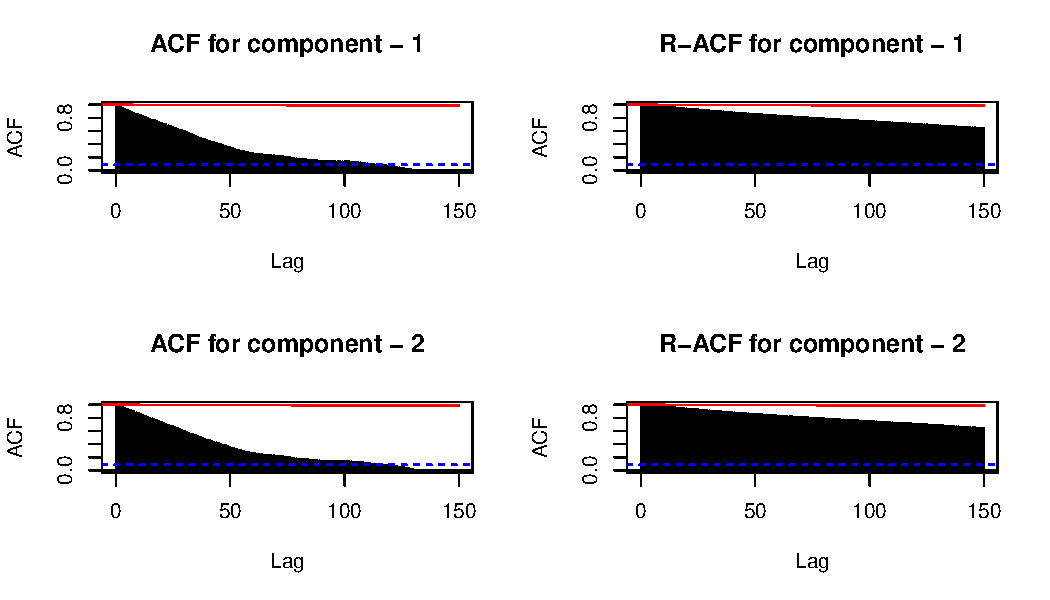
\includegraphics[width=.8\linewidth]{var-acf_5e2.pdf}
  \caption{$n = 500$}
  \label{subfig:acf-500}
\end{subfigure}\\
\begin{subfigure}{\textwidth}
  \centering
  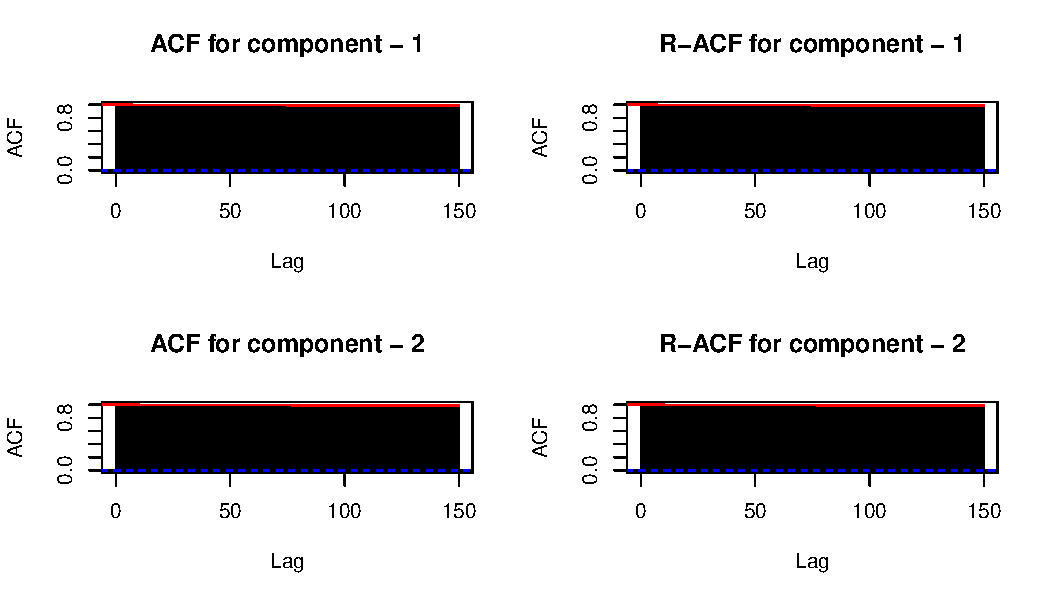
\includegraphics[width=.8\linewidth]{var-acf_5e4.pdf}
  \caption{$n = 5*10^4$}
  \label{subfig:acf-5e4}
\end{subfigure}
\caption{Autocorrelation plot for ACF and R-ACF for first chain out of two parallel Markov chains. First column corresponds to ACF calculated using arithmetic mean of first Markov chain and the second column corresponds to the one calculated using global mean of two Markov chains.(a): $n = 500$, not converged yet; (b): $n = 5 \times 10^4$, converged}
\label{fig:var_acf_ccf}
\end{figure}

The bias for R-ACF is similar to the bias of sample autocovariance estimator in case of single chain except for a few small order terms that shall be later addressed in theorem \ref{th:RAC_expec}. Before getting to the bias results for $\hat{\Gamma}_{RAV}(k)$ for any lag k, we introduce an additional notation. For $q \geq 1$, we define
\[
\Phi^{(q)} = \sum\limits_{-\infty}^{\infty}\abs{k}^q \|\Gamma(k)\|
\]
We denote $\Phi^{(1)} \textrm{ by } \Phi$. 
\begin{theorem} \label{th:RAC_expec}
   \[
   \mathbb{E}[\hat{\Gamma}_{RAC}(k)] = \left(1- \dfrac{|k|}{n}\right)\left(\Gamma(k) - \dfrac{\Sigma}{mn} - \dfrac{\Phi}{mn^2}\right)  + \dfrac{2(m-1)}{m}\dfrac{\abs{k}}{n^2} \left(\Sigma - \sum_{h=0}^{n-1}\Gamma(h)\right) + o(n^{-2})
   \]
\end{theorem}

\begin{proof}
 The estimator for autocovariance with divisor $n$ is suggested by \cite{parzen1961approach} for its lesser mean square error despite having greater bias than the unbiased estimator with an $n - \abs{k}$ divisor. 
 We know that $\hat{\Gamma}_s(k)$ is asymptotically unbiased with a $o(1)$ bias term that remains fixed for any $k$. The bias term is given by \cite{priestley1981spectral} as 
 
 \begin{equation} \label{eq:priestly}
     \mathbb{E}[\hat{\Gamma}(k) = \left(1- \dfrac{\abs{k}}{n}\right)\left(\Gamma(k) - \Var{(\bar{X})}
 \right)
 \end{equation}
 
By proposition 1 in \cite{song1995optimal} 
\begin{equation} \label{eq:song}
\Var(\overline{X}) = \dfrac{\Sigma}{n} + \dfrac{\Phi}{n^2} + o(n^{-2})
\end{equation}

As a consequence, if $\Var(\bar{X})$ is finite, then $\Var(\bar{X}) \to 0 \textrm{ as } n \to \infty$. We can break $\hat{\Gamma}_{RAC}$ into four parts for all $k \geq 1$ as:
 \[
 \hat{\Gamma}_{RAC} =  \dfrac{1}{m}\sum_{s=1}^{m}\hat{\Gamma}_s(k) - \dfrac{1}{mn}\sum_{s=1}^{m}\sum_{t=1}^{|k|}A_{st}^T - \dfrac{1}{mn}\sum_{s=1}^{m}\sum_{t=n-|k|+1}^{n}A_{st} + \dfrac{n-|k|}{mn}\sum_{s=1}^{m}(\overline{X_s}-\overline{\overline{X}})(\overline{X_s}-\overline{\overline{X}})^T
 \]
 
where $A_{st} = (X_{st}-\overline{X}_s)(\overline{X}_s - \overline{\overline{X}})^T$\\
The expectation value of the first term is given by equation \ref{eq:priestly} and \ref{eq:song} while the other three terms contribute $o(1)$ terms. The complete proof evaluating the expectation values of last three terms can be found in Appendix subsection \ref{appendix:bias}.
\end{proof}

\begin{remark} \label{rmrk:exp_racf_minus_acf}
Using theorem \ref{th:RAC_expec} and equation \ref{eq:priestly},
\[
\mathbb{E}[\hat{\Gamma}_{RAC}(k) - \hat{\Gamma}(k)] = \dfrac{\abs{k}}{n}\left(1 - \dfrac{1}{m}\right)\left(\dfrac{\Sigma}{n} + \dfrac{\Phi}{n^2}\right) + \dfrac{2(m-1)}{m}\dfrac{\abs{k}}{n^2} \left(\Sigma - \sum_{h=0}^{n-1}\Gamma(h)\right) + o(n^{-2})
\]
We know that the sample autocovariance $\hat{\Gamma}(k)$ underestimates the truth due to a negative bias of $\abs{k}\Gamma(k)/n$ for finite $n$. However, in practice, it is preferred to overestimate the autocovariance for finite $n$ than to underestimate it in order to have a more realistic idea about the correlation in a Markov chain at a particular lag.  Note that the RHS in the above expression is positive. As a consequence, R-ACF will counter this negative bias and give more reliable estimates for ACF. 

\end{remark}

\begin{corollary} \label{cor:lag0_expectation}, 
\[
\mathbb{E}[\hat{\Gamma}_{RAC}(0)] = \Gamma(0) + \dfrac{\Sigma}{mn} + \dfrac{\Phi}{mn^2} + o(n^{-2})
\]
\end{corollary}

\begin{proof}
 The proof is in Appendix subsection \ref{appendix:bias}.
\end{proof}

\section{Variance Estimators for multiple Markov chains} \label{sec:variance_est}

Let $\{X_t\}_{t \geq 1}$ be a stochastic process. Denote lag-k autocovariance matrix by $\Gamma(k)$, which is given by,

\[
\Gamma(k) = \Gamma(-k) = \E[(X_t - \E[X])(X_{t+k} - \E[X])^T]
\]

Recall that $\hat{\Gamma}(k)$ is the empirical autocovariance function given by 

\[
\hat{\Gamma}(k) = \dfrac{1}{n}\sum_{t=1}^{n-\abs{k}}(X_t - \overline{X})(X_{t + \abs{k}} - \overline{X})^T
\]

The spectral variance estimator is the weighted and truncated sum of lag-k autocovariances, given by:

\[
\hat{\Sigma}_{SV} &= \sum_{k=-b_n+1}^{b_n-1}w_n\left(\dfrac{k}{b_n}\right)\hat{\Gamma}_n(k)
\]

where $w_n(.)$ is the lag window and $b_n$ is the truncation point.\\

 Consider $m$ Markov chains where $\overline{X}_s$, $\hat{\Gamma}_s(k)$ and $\hat{\Sigma}_{SV, s}$ are the sample mean, sample lag-k autocovariance and spectral variance estimators respectively for $s^{th}$ Markov chain, $s\in {1,...,m}$. We will consider two estimators for spectral variance calculations using multiple Markov chains.

\subsection{Average Spectral Variance } \label{sec:asv}

Recall that for $s^{th}$ Markov chain, the spectral variance estimator is given by,

\begin{align*}
    \hat{\Sigma}_{SV,s} &= \sum_{k=-b_n+1}^{b_n-1}w_n\left(\dfrac{k}{b_n}\right)\hat{\Gamma}_s(k)\\
    \hat{\Gamma}_s(k) &= \dfrac{1}{n}\sum_{t=1}^{n-k}(X_{st}-\overline{X_s})(X_{s(t+k)}-\overline{X_s})^T
\end{align*}

The average spectral variance ($\Sigma_{ASV}$) is computed by averaging the SV estimates from all $m$ Markov chains.

\[
\hat{\Sigma}_{ASV} = \dfrac{1}{m}\sum_{s=1}^{m}\hat{\Sigma}_{SV,s}
\]

\subsection{Replicated Spectral Variance } \label{sec:rsv}

Now we introduce the Replicated Spectral Variance Estimator (RSV). $\hat{\Gamma}_{RAC,s}(k)$ is the sample replicated lag-k autocovariance estimator for the $s^{th}$ MC using overall mean $(\overline{\overline{X}})$ instead of $\overline{X}_s$ for centering. We construct an RSV estimator $\hat{\Sigma}_{RSV} $ using this replicated version of autocovariance estimator. Consider, 

\begin{align*}
    \hat{\Sigma}_{RSV,s} &= \sum_{k=-b_n+1}^{b_n-1}w_n\left(\dfrac{k}{b_n}\right)\hat{\Gamma}_{RAC,s}(k)\\
\end{align*}
$$\hat{\Sigma}_{RSV} &=  \dfrac{1}{m}\sum_{s=1}^{m}\hat{\Sigma}_{RSV,s}$$

The RSV estimator centers the data around the global mean. We are interested in proving the strong consistency, finding the bias and variance of RSV. 

\begin{ass}[Strong Invariance Principle (SIP)] \label{ass:sip}
    We assume the SIP holds for the Markov chain. Here $\{X_t\}_{t\geq 1}$ is the stochastic process that follows SIP with mean $\mu = \mathbb{E}[X]$. Let $\|.\|$ denote the Euclidean norm. Through SIP, there exists a $p \times p$ lower triangular matrix L, an increasing function $\psi$ on the integers, a finite random variable D, and a  sufficiently rich probability space such that, with probability 1, \\
  $$\left\|\sum_{t=1}^{n}X_t - n\mu - LB(n)\right\| < D\psi(n)$$
  
  Let $\{B(n)\}_{n\geq 0}$ denotes a standard p-dim Brownian motion and $B^{(i)}$ denotes its $i^{th}$ component. As shown in the results \cite{kuelbs1980almost}, SIP will hold for $\psi(n) = n^{1/2 - \lambda, \; \lambda > 0}$ for Markov chains commonly encountered in MCMC settings. We know that $\psi(n)$ is an inherent property of the stochastic process that satisfies the CLT. This implies that $\psi(n)$ is at least $o(\sqrt{n})$. Using Law of Iterative Logarithms (LIL), a tighter bound for $\psi(n)$ is given by \cite{stra:1964} as $\mathcal{O}(\sqrt{n\log \log n})$.
\end{ass}

\bigskip

\begin{ass} \label{ass:sve_consis} We assume that all the conditions given by \cite{vats:fleg:jon:2018} for strong consistency of the spectral variance estimator hold true. As a consequence, 
\[
\hat{\Sigma}_{SV,s} \xrightarrow{a.s.} \Sigma \textrm{ as } n \to \infty \;\; \forall s \in \{1,..., m\}
\]
\end{ass}

\bigskip

We are going to consider a class of pseudo spectral variance estimator denoted by $\tilde{\Sigma}$ which uses data centered around the unobserved actual mean $\mu$. Such pseudo covariance estimator and autocovariance estimator for the $j^{th}$ chain is denoted by $\tilde{\Sigma}_s$ and $\tilde{\Gamma}_s$ respectively.

\begin{align*}
    \tilde{\Sigma}_s &= \sum_{k=-b_n+1}^{b_n-1}w_n\left(\dfrac{k}{b_n}\right)\tilde{\Gamma}_s(k)\\
    \tilde{\Gamma}_s(k) &= \dfrac{1}{n}\sum_{t=1}^{n-|k|}(X_{st}-\mu)(X_{s(t+k)}-\mu)^T
\end{align*}

The average pseudo spectral variance estimator (APSVE) is given by

\[
\tilde{\Sigma} = \dfrac{1}{m}\sum\limits_{s=1}^{m}\tilde{\Sigma}_s
\]

\bigskip
\begin{theorem}
\label{th:consistency}
 Let the Assumptions \ref{ass:sip},\ref{ass:sve_consis} hold and $\dfrac{b_n \log \log n}{n} \to 0 \textrm{ as } n \to \infty$, then $\hat{\Sigma}_{RSV} \to \Sigma$ with probability 1, as $n \to \infty$.
\end{theorem} 

\begin{proof}
We complete the proof by showing that $\hat{\Sigma}_{RSV}^{ij} - \tilde{\Sigma}^{ij}$ converges to 0 almost surely for all $i,j \in \{1,...,p\}$ and $\tilde{\Sigma}^{ij} \to \Sigma^{ij}$ with probability 1 as $n \to \infty$. We will show that 

\[
\hat{\Sigma}_{RSV}^{ij} - \tilde{\Sigma}^{ij} = g_1(n)D^2 + g_2(n)D + g_3(n)
\]
where $D$ is the finite random variable associated with SIP. We will show that\\

\begin{align*}
    g_1(n) &= (4+C_1)\dfrac{b_n \psi^2(n)}{n^2} - 4\dfrac{\psi^2(n)}{n^2}\\
    g_2(n) &= 2\sqrt{2}\|L\|p^{1/2}(1+\epsilon)\left[(4+C_1)\dfrac{b_n\psi(n)\sqrt{n\log \log n}}{n^2} - 4\dfrac{\psi(n)\sqrt{n\log \log n}}{n^2}\right]\\
    g_3(n) &= \|L\|^2 p (1+\epsilon)^2\left[(4+C_1)\dfrac{b_n \log\log n}{n} - 4 \dfrac{\log \log n}{n}\right]
\end{align*}

Using $\psi(n) = \mathcal{O}(\sqrt{n \log \log n}),\; b_n = o(n), \textrm{ and } b_n \log \log n = o(n)$, we will finally we prove that $g_1(n), g_2(n), g_3(n) \to 0$ with probability 1, as $n \to \infty$. The proof is in Appendix subsection \ref{appendix:strong_consis}
\end{proof}

\bigskip

We are interested in the finding the bias for RSV estimator as a function of $n$. The proof below applies to all the important range of lag windows $w_n(x)$; where $w_n(x)$ is a continuous, even fnction with $w_n(0)=1, \abs{w_n(x)} < c$, and $\int_{-\infty}^{\infty}w_n^2(x)dx < \infty$. Define

\[
W_n = \dfrac{1}{2\pi}\sum_{k=-b_n+1}^{b_n-1}w_n\left(\dfrac{k}{b_n}\right)
\]

We have $W_n < \infty$ for all the important lag windows.

\begin{ass} \label{ass:bias}
    Let $\Gamma_s(k)$ be the lag-k autocovariance for $s^{th}$ Markov chain and $w_n(x)$ be the lag window. We assume that there exists a $q \geq 0$ such that
    \begin{enumerate} [a.]
        \item $\sum\limits_{-\infty}^{\infty}\abs{k}^q \|\Gamma(k)\| < \infty$
        \item $\lim _{x \to 0}\dfrac{1 - w_n(x)}{\abs{x}^q} = k_q < \infty$
        \item $\dfrac{b_n^q}{n} \to 0$ as $n \to \infty$
    \end{enumerate}
    
    If $k_q$ is finite for some $q_o$, then it is zero for $q < q_0$. $q$ is taken to be the largest number satisfying the first two conditions above.
\end{ass}


\begin{theorem}\label{th:rsv_bias}
The limiting bias of replicated spectral variance is given by:
\[
 \lim_{n \to \infty}b_n^q\mathbb{E}[\hat{\Sigma}_{RSV} - \Sigma] = -k_q\Phi^{(q)}
 \]
\end{theorem}

\begin{proof}

\[
\mathbb{E}[\hat{\Sigma}_{RSV} - \Sigma] = \sum_{k=-b_n+1}^{b_n-1} w\left(\dfrac{|k|}{b_n}\right)\mathbb{E}[\hat{\Gamma}_{RAC}(k)]-\sum_{k=-\infty}^{\infty}\Gamma(k)
\]

Using theorem \ref{th:RAC_expec}, we can write the expectation of $\hat{\Gamma}_{RAC}$ as  a sum of equation \ref{eq:priestly} and some small order terms.
The proof is given in the Appendix subsection \ref{appendix:bias}.
\end{proof}


\begin{ass} \label{ass:variance_cal}
Let $\{X_{st}\}_{t \geq 1}$ be the $s^{th}$ Markov chain for which SIP holds. 
\begin{enumerate}[a.]
    \item $\E[D^4] < \infty$ where D is a finite random variable associated with the SIP
    \item $\E[X^4] < \infty$ where $\{X\}$ is the stochastic process
\end{enumerate}
\end{ass}

\bigskip

\begin{theorem} \label{th:rsv_variance}
 If Assumption \ref{ass:variance_cal} hold, $\dfrac{n}{b_n}\Var\hat{\Sigma}_{RSV}^{ij} = [\Sigma_{ii}\Sigma_{jj} + \Sigma_{ij}^2]\int_{-\infty}^{\infty}w(x)^2dx  + o(1)$.
\end{theorem}

\begin{proof}
Recall that $\tilde{\Sigma}$ is the averaged pseudo spectral variance estimator which uses the unobserved mean. Further, let $\tilde{\Sigma}^{ij}$ be the $(i,j)^{th}$ element of this matrix. We will prove that the variance of $\hat{\Sigma}_{RSV} \textrm{ and } \tilde{\Sigma}$ are equivalent for large sample sizes. The proof is in Appendix subsection \ref{appendix:variance}
\end{proof}


\section{Effective sample size} \label{sec:ess}

Estimating the MCSE is crucial for determining when to terminate the simulations. The existing stopping rules rely on the strong consistency of the estimator of $\Sigma$. We will use the \textit{relative standard deviation fixed-volume sequential stopping rule} proposed in \cite{vats2019multivariate} when multivariate Markov chain central limit theorem holds. This stopping rule terminates the simulations on the basis of size of confidence interval relative to inherent variability in the target distribution. It terminates after the total number of samples, i.e. $mn$ exceed some pre-specified $n^*$ iterations to prevent pre-mature termination due to bad estimates of $\Sigma$ and $\Lambda$. The rule is given by

\[
\textrm{Volume of confidence region}^{1/p} + n^{-1} < \epsilon \abs{\Lambda_n}^{1/2p} 
\]

where $\epsilon$ is the tolerance level, $\abs{.}$ denotes the determinant and $\Lambda_n$ is the sample covariance matrix given by

\[
\dfrac{1}{mn-1}\sum_{s=1}^{m}\sum_{t=1}^{n}(X_{st} - \overline{\overline{X}})(X_{st} - \overline{\overline{X}})^T
\]

The determinant of Monte Carlo standard error is called generalized variance in  \cite{wilks1932certain} and gives a metric for volume of confidence interval. \cite{vats2019multivariate} showed that if the estimator for $\Sigma$ is strongly consistent, the stopping rule is asymptotically valid, in that the confidence regions created at termination have the right coverage probability as $\epsilon \to 0$. Since $\hat{\Sigma}_{RSV}$ is a strongly consistent estimator of $\Sigma$, w

\[
\abs{\hat{\Sigma}_{RSV}}^{1/p} + (mn)^{-1} < \epsilon \abs{\Lambda_{mn}}^{1/2p}
\]

Another way to get more accurate stopping rule is to use RSV estimator for estimating Effective Sample Size (ESS) in multivariate settings. RSV estimator better captures the standard error of target distribution by considering the global sample mean across the Markov chains; which might otherwise get lost when considering a single localized slowly mixing Markov chain. We therefore define our ESS rule as

\[
ESS = mn\left(\dfrac{\abs{\Lambda_{mn}}}{\abs{\hat{\Sigma}_{RSV}}}\right)^{1/p}
\]

When there is no correlation in Markov chain $\hat{\Sigma}_{RSV} = \Lambda_{mn}$ and therefore, ESS = $n$. Both the rules involve the ratio of generalized variances and therefore the relative standard deviation fixed-volume sequential stopping rule is asymptotically equivalent to stopping when ESS is greater than $W_{p,\alpha,\epsilon}$ which depends on dimension of state-space, level of confidence of the confidence region, and the relative precision required. 

\section{Examples} \label{sec:examples}

In the following examples we compare the performance of asymptotic variance estimators (ASVE and RSVE) for Markov chain CLT. We will successfully illustrate that the replicated spectral variance estimator performs better than the average spectral variance estimator in terms of ESS calculations, coverage probabilities , and sample distribution of $\Sigma$. We will also show that in case of nicely mixing Markov chains, these estimators give almost equivalent results. As a consequence, while out replicated version of variance estimator is better in cases where the Markov chains do not explore the entire sample space in finite time, it is harmless to be used in cases where they do.  
{\color{red}about this new FFT based method for faster RSVE calculations}

\subsection{Vector Autoregressive Process} \label{ex:var}

We examine the vector autoregressive process of order 1 (VAR(1)) where the true autocovariance in known in closed form. We have already illustrated the better performance of R-ACF over traditional ACF on a slowly mixing VAR(1) process in Figure \ref{fig:var_acf_ccf}. Here we will examine the performance of RSV estimator on the same process. Consider a p-dimensional VAR(1) process $\{X_t\}_{t \geq 1}$ such that

\[
X_t = \Phi X_{t-1} + \epsilon_t
\]

where $X_t \in \mathbb{R}^p$, $\Phi $ is a $p \times p $ matrix, $ \epsilon_t \overset{i.i.d.}{\sim} N(0, \Omega)$, and $\Omega$ is a positive definite $p \times p$ matrix. The invariant distribution for this Markov chain is $N(0, \Psi)$ where $\Vec{\Psi} = (I_{p^2} - \Phi \otimes \Phi)\Vec{\Omega}$. The lag-k autocovariance can be calculated easily for $k >0$ as

\begin{align*}
    \Gamma(k) &= \Phi^k\Psi\\
    \Gamma(-k) &= \Psi(\Phi^T)^k
\end{align*}

The Markov chain is geometrically ergodic when the spectral norm of $\Phi$ is less than 1 (\cite{10.2307/1427459}). The CLT holds for the invariant distribution, therefore, $\Sigma$ exists and is given by

\[
\Sigma = (1 - \Phi)^{-1}\Psi + \Psi(1 - \Phi^T)^{-1} - \Psi
\]

Let $\phi_{max}$ be the largest absolute eigenvalue of $\Phi$ such that $\abs{\phi_{max}} < 1$. The larger it is, the slower the Markov chain mixes. For our case, we require a slowly mixing VAR(1) process. We consider a bivariate example with $\phi_{max} = 0.9999$. We run five parallel Markov chains with their starting points evenly distributed about the center of invariant distribution. Figure \ref{subfig:var-sp_500} shows that for the first 500 samples, the chains have not explored the sample space well unlike Figure \ref{subfig:var-sp_50000} with $5\cdot 10^4$ samples.  

\begin{figure}[h]
    \centering
    \begin{subfigure}[h]{0.4\textwidth}
         \centering
         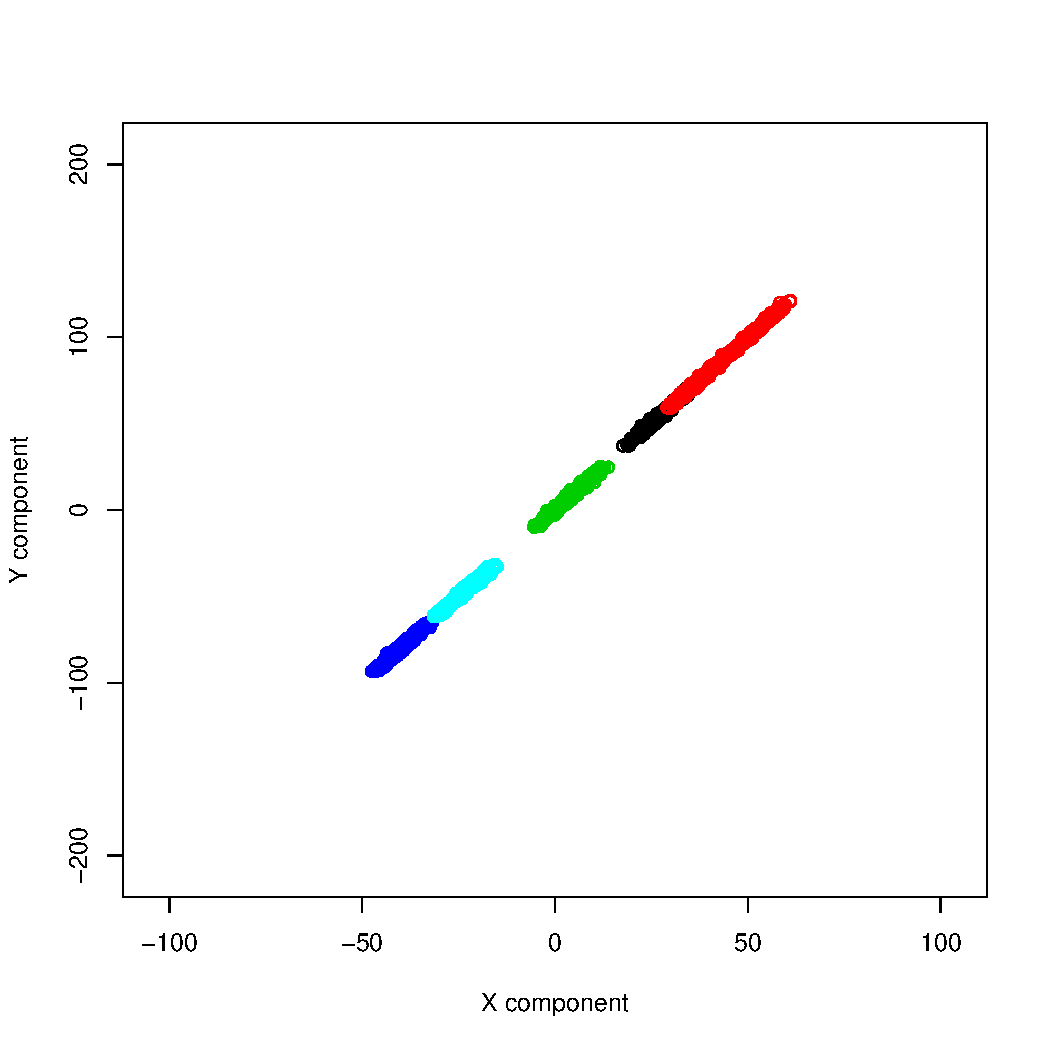
\includegraphics[width=\textwidth]{var-sp_5e2.pdf}
         \caption{$n = 500$}
         \label{subfig:var-sp_500}
     \end{subfigure}
     \begin{subfigure}[h]{0.4\textwidth}
         \centering
         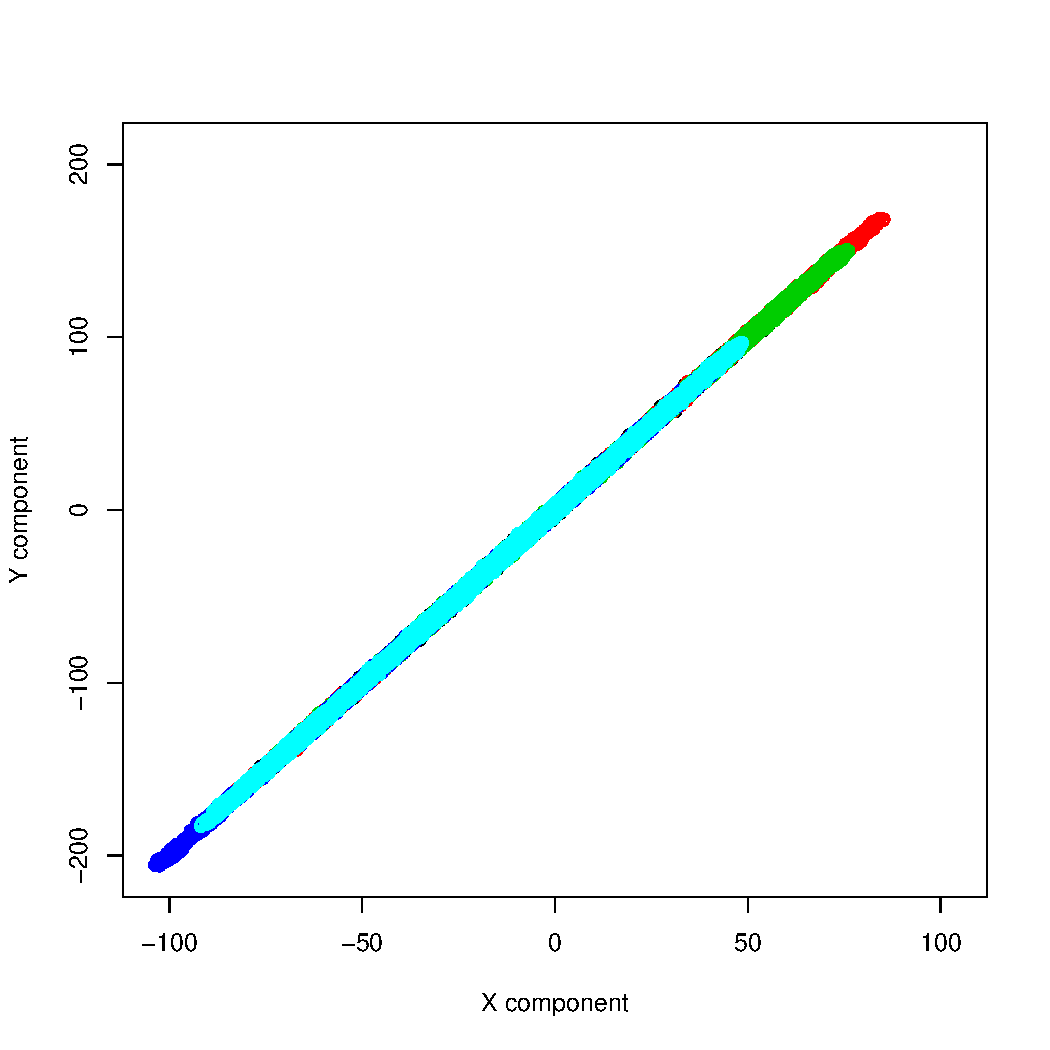
\includegraphics[width=\textwidth]{var-sp_5e4.pdf}
         \caption{$n = 5 \times 10^4$}
         \label{subfig:var-sp_50000}
     \end{subfigure}
    \caption{Scatter plot of five Markov chains for different sample sizes.}
    \label{fig:var-sp}
\end{figure}

\begin{figure}[h]
    \centering
    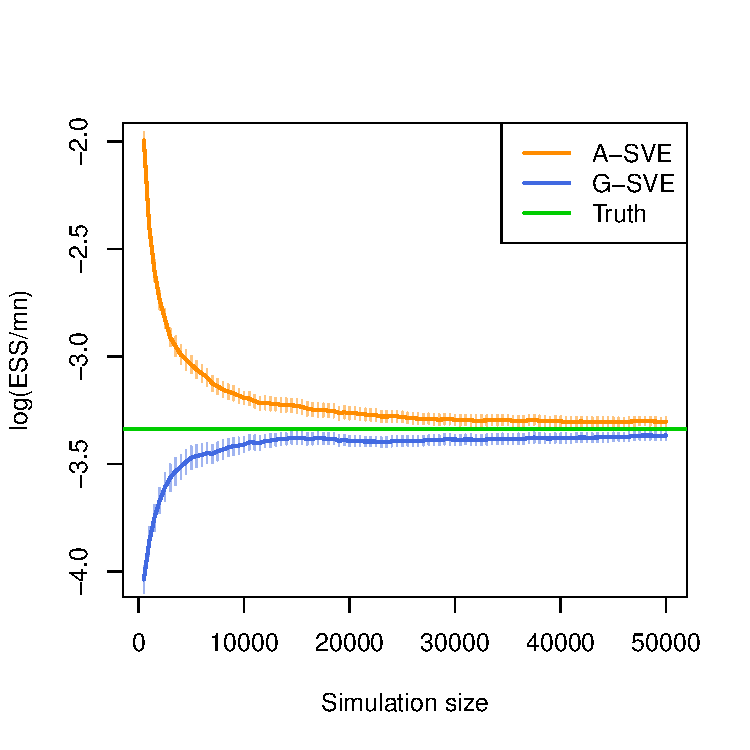
\includegraphics[width = .5\textwidth]{plots/var-ess.pdf}
    \caption{Running plots for $\hat{ESS}/mn$ calculated using ASV (black) and RSV (blue). The true $ESS/mn$ (red) is known.}
    \label{fig:var-ess}
\end{figure}


\subsection{Boomerang Distribution} \label{ex:boomerang}

We will use a bivariate bi-modal distribution introduced by \cite{gelman1991note} which has Gaussian conditional distributions in both directions. This allows us to sample parallel Markov chains using the Gibbs sampler. Let $x$ and $y$ be two random variable that are jointly distributed as 

\[
f(x, y) \propto \exp\left(-\dfrac{1}{2}[Ax^2y^2 + x^2 + y^2 -2Bxy  -2C_1x - 2C_2y]\right)
\]

The conditional distribution of $x$ given $y$ and vice versa is a normal distribution given by:

\begin{align*}
    x_1 \mid x_2 &\sim N\left(\dfrac{Bx_2 + C_1}{Ax_2^2 + 1}, \dfrac{1}{Ax_2^2 + 1}\right)\\
    x_2 \mid x_1 &\sim N\left(\dfrac{Bx_1 + C_2}{Ax_1^2 + 1}, \dfrac{1}{Ax_1^2 + 1}\right)
\end{align*}

We use a carefully chosen parameterization of $A = 1,\; B = 3,\; C = 8$ which ensures bimodality for our purpose.  Let $n$ be the number of samples in each chain and $m$ be the number of Markov chain replications. Finding the actual mean of this distribution in closed form is difficult. Therefore, we use numerical integration with fine tuning to calculate it. We sample two parallel Markov chains with well-separated starting values. 

\begin{figure}[h]
    \centering
    \begin{subfigure}[h]{.4\textwidth}
        \centering
        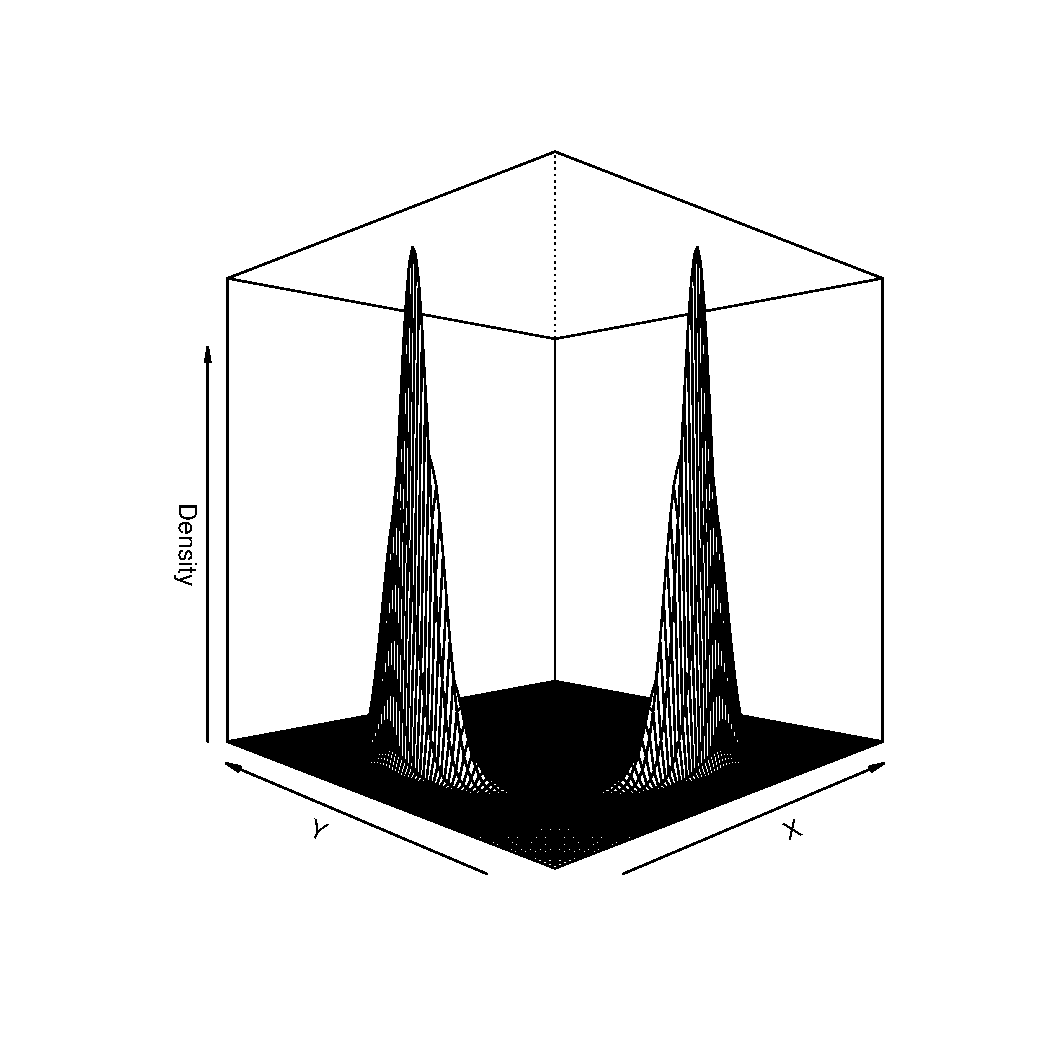
\includegraphics[width = \textwidth]{plots/boom-pers_1_3_8.pdf}
        \caption{$A = 1, B = 3, C = 8$}
        \label{subfig:boom-pers_1_3_8}
    \end{subfigure}
    \begin{subfigure}[h]{.4\textwidth}
        \centering
        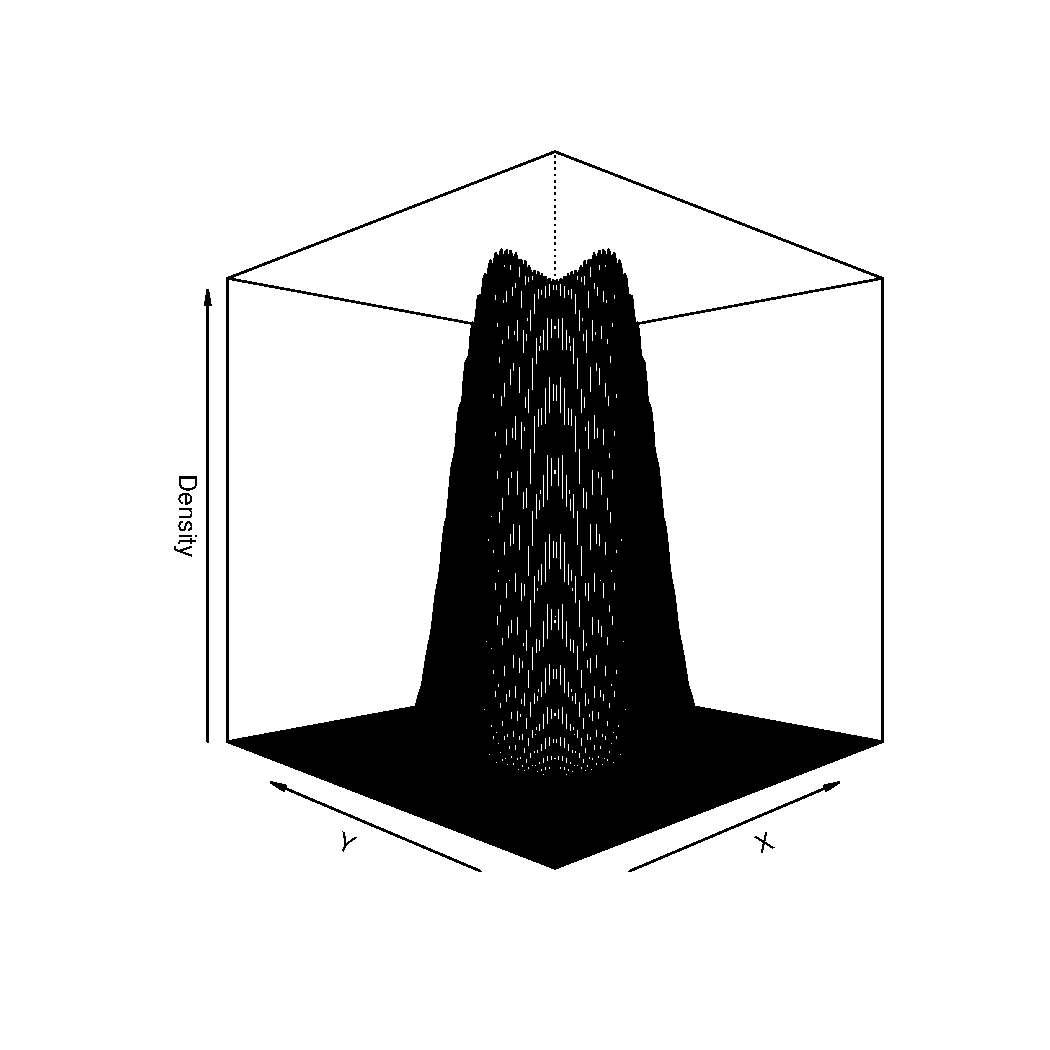
\includegraphics[width = \textwidth]{plots/boom-pers_1_10_7.pdf}
        \caption{$A = 1, B = 10, C = 7$}
        \label{subfig:boom-pers_1_10_7}
    \end{subfigure}
    \caption{Perspective plots of the target distribution for two different parameterizations.}
   \label{fig:3d_plot}
\end{figure}

\begin{figure}[h]
    \centering
    \begin{subfigure}[h]{.4\textwidth}
      \centering
      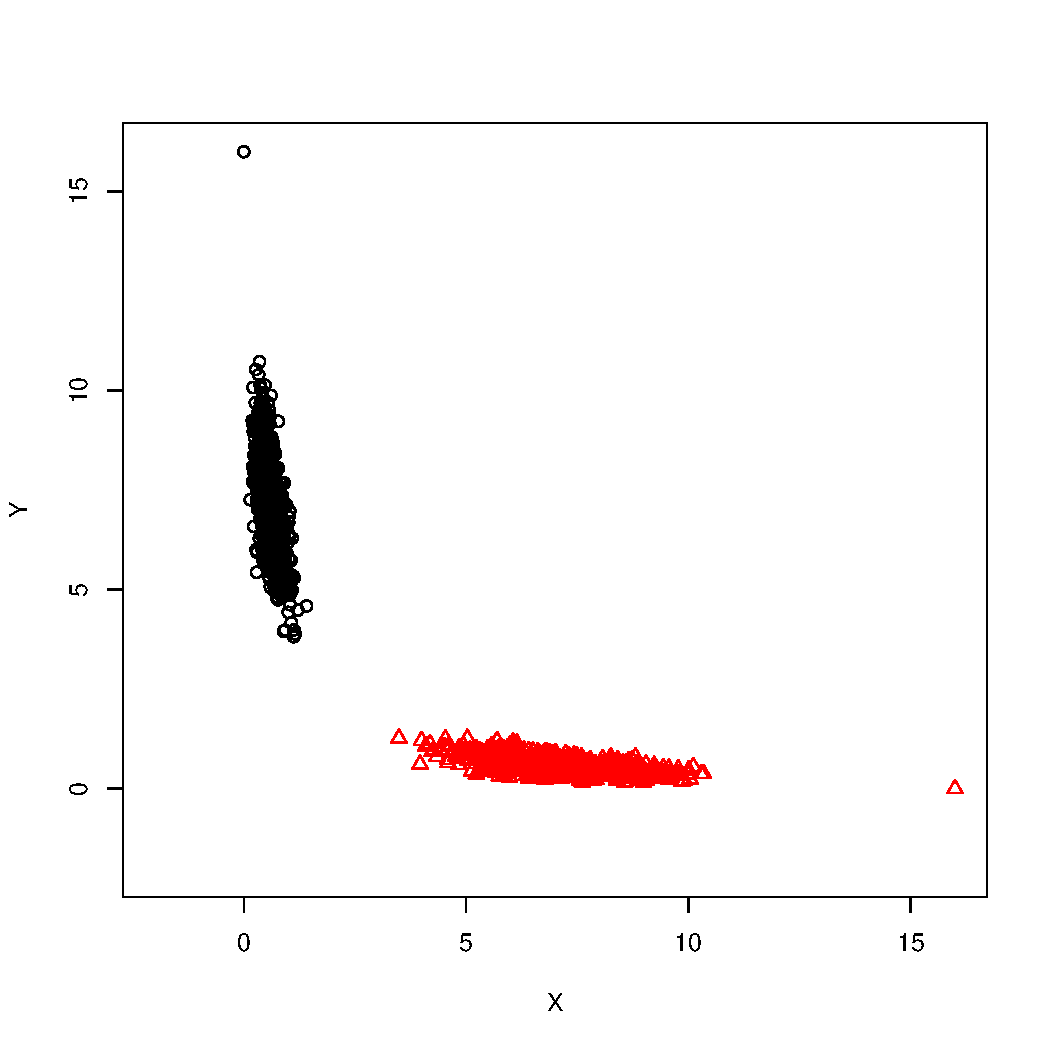
\includegraphics[width = \textwidth]{plots/boom-sp_1e3.pdf}
      \caption{$n = 1000$}
      \label{subfig:boom-sp_1e3}
    \end{subfigure}
    \begin{subfigure}[h]{.4\textwidth}
      \centering
      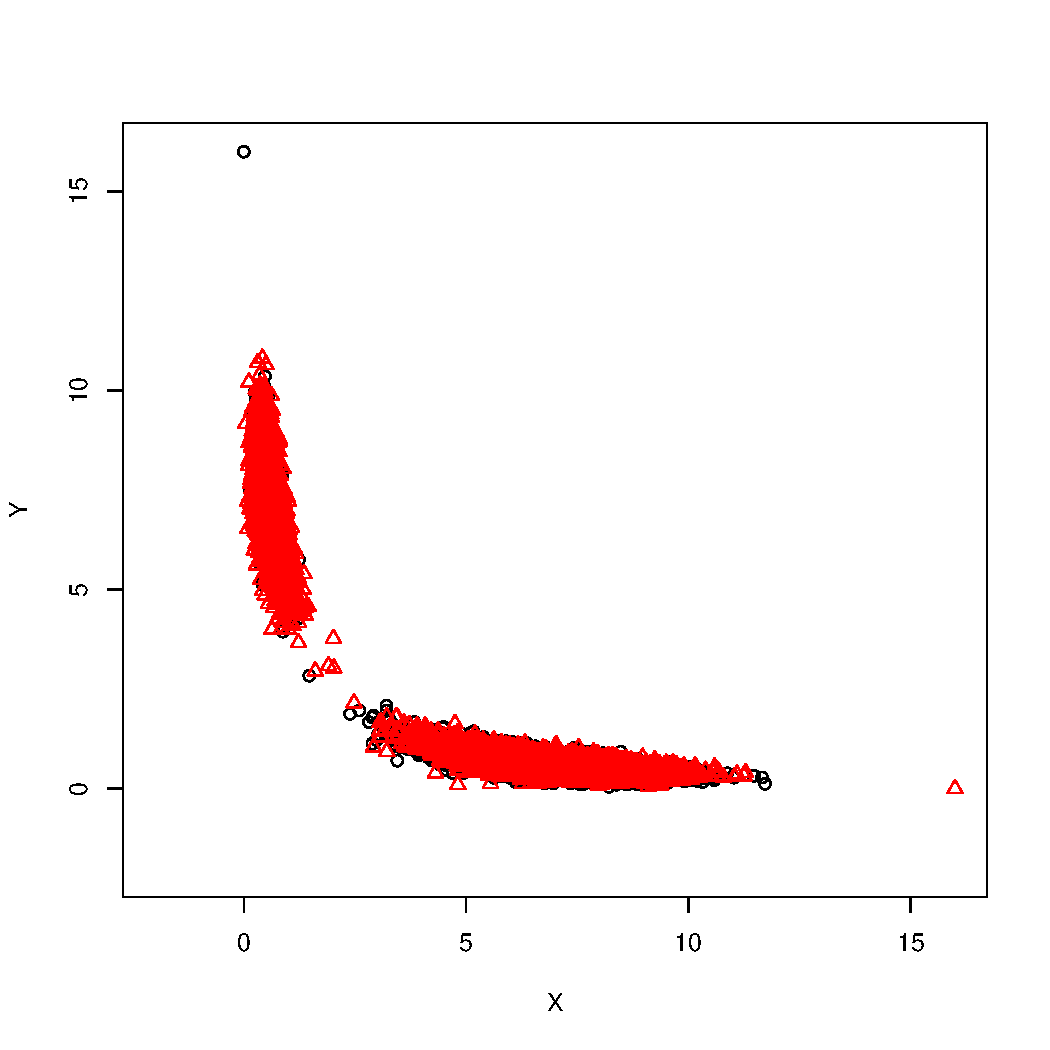
\includegraphics[width = \textwidth]{plots/boom-sp_1e4.pdf}
      \caption{$n = 10,000$}
      \label{boom-sp_1e4}
    \end{subfigure}
    \caption{The scatter plots for two parallel Markov chains. (a): Both the chains are stuck in one of the mode (b): Both the chains have travelled and explored both the modes.}
    \label{fig:boom-sp}
\end{figure}

In Figure \ref{fig:boom-sp}, we demonstrate the "sticky" nature of the Markov chains. For the first thousand samples, both the chains are oblivious of the existence of another mode. By ten thousand samples, both the Markov chains have explored the two modes. This property will affect the single chain estimators like ACF. In Figure \ref{subfig:boom-acf_1e3}, the ACF is severely underestimated because the chain-1 has not jumped to the other mode. Whereas, in Figure \ref{subfig:boom-acf_1e4}, both ACF and R-ACF give almost similar results indicating that both modes have been explored by chain-1.   

\begin{figure}[h]
    \centering
    \begin{subfigure}[h]{.7\textwidth}
      \centering
      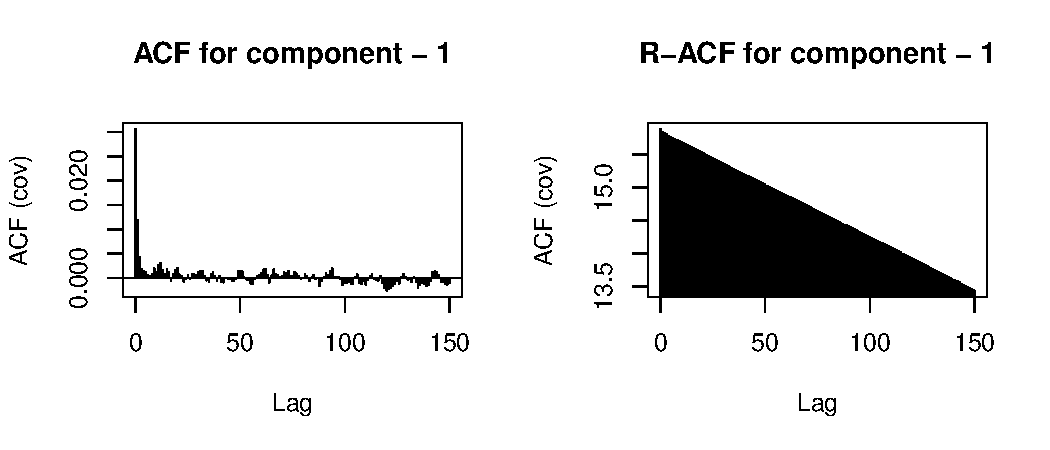
\includegraphics[width = \textwidth]{boom-acf_1e3.pdf}
      \caption{$n = 1000$}
      \label{subfig:boom-acf_1e3}
    \end{subfigure}
    \begin{subfigure}[h]{.7\textwidth}
      \centering
      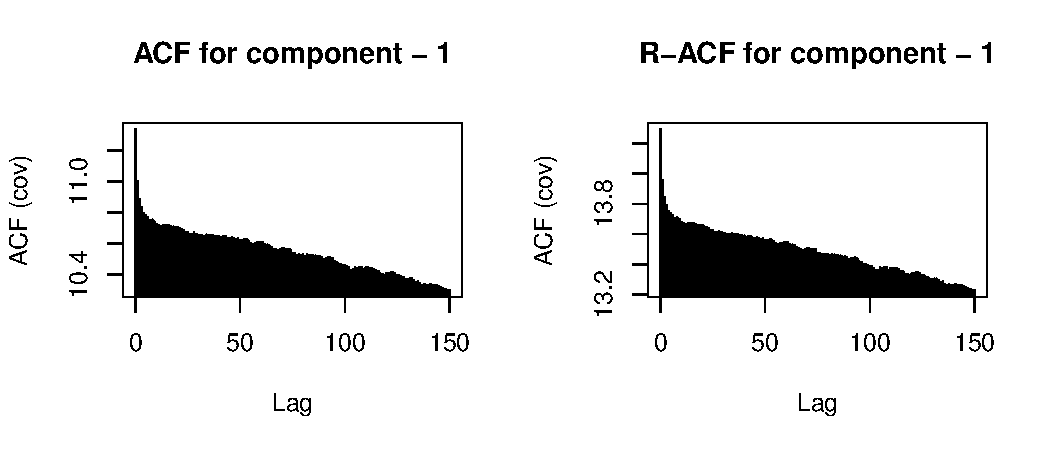
\includegraphics[width = \textwidth]{boom-acf_1e4.pdf}
      \caption{$n = 10,000$}
      \label{subfig:boom-acf_1e4}
    \end{subfigure}
    \caption{ACF and R-ACF for component-1 of chain-1 at two different sample sizes. }
    \label{fig:boom-acf}
\end{figure}

We also run five parallel Markov chains with well-separated starting points. In Table \ref{table:boom-coverage_1_3_8}, we give the coverage probabilities for $95 \%$ confidence interval for both the estimator. We can see that the RSVE gives better coverage probabilities for all the $n$. For smaller sample size, the coverage probability of RSVE is significantly higher than ASVE. As the number of samples per chain increases, they start coming closer due to the strong consistency of both the estimators.

\begin{table}[h]
\centering
    \begin{tabular}{p{1cm}|p{2cm}|p{2cm}|p{2cm}|p{2cm}}
    \toprule
        n & \multicolumn{2}{|c|}{$m = 2$} & \multicolumn{2}{|c|}{$m=5$}\\
        \hline
        & ASV & RSV & ASV & RSV\\
        \hline
        $10^3$ & 0.612 & 0.689 & 0.602 & 0.753   \\
        $2\cdot10^3$ & 0.693 & 0.751 & 0.735 & 0.827 \\
        $5 \cdot 10^3$  & 0.826 & 0.854 & 0.847 & 0.880 \\
        $10^4$  & 0.862 & 0.868 & 0.884 & 0.907 \\
        $2 \cdot 10^4$ & 0.899 & 0.906 & 0.922 & 0.934 &  &  \\
    \bottomrule
    \end{tabular}
    \caption{Coverage probabilities for parameter values $A = 1,\; B = 3,\; C = 8$. }
    \label{table:boom-coverage_1_3_8}
\end{table}

A good estimate of ESS is crucial to determine when to stop the simulations. We can see in Figure \ref{fig:run_ess} that for the first few thousand samples, ASVE gives misleadingly higher $\hat{ESS}/mn$ than RSVE. This can cause us to stop the sampling before the sample space has been explored by the chains. The inferences derived from this chain would then be severely non-informative.

\begin{figure}[h]
    \centering
    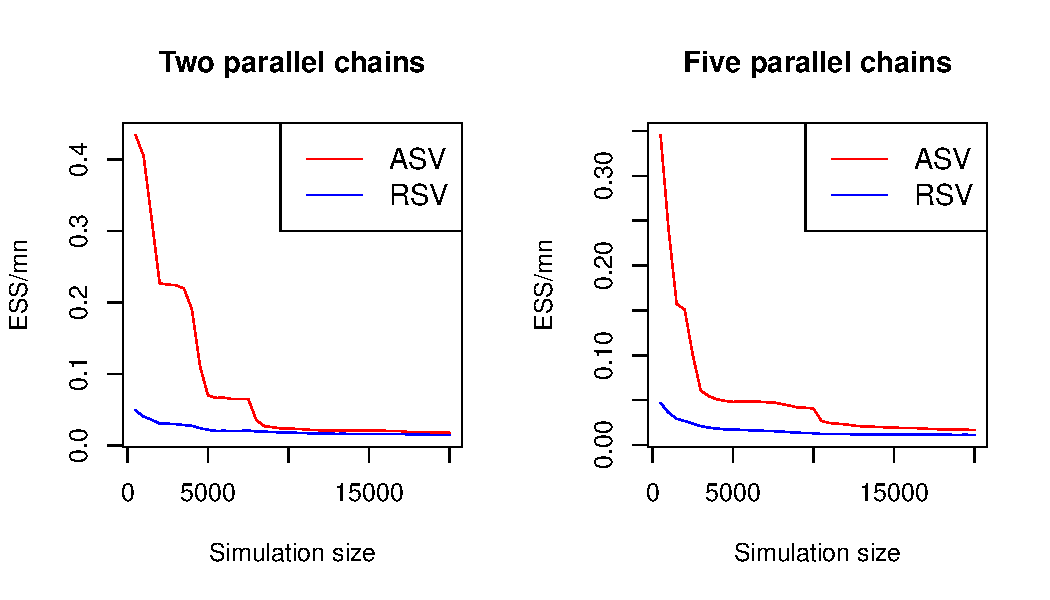
\includegraphics[width = .7\textwidth]{plots/boom-ess.pdf}
    \caption{Running plot for $\hat{ESS}/mn$ using ASV and RSV calculated for two chains (left) and five chains (right). The parameters for target distribution are $A == 1, \; B = 3, \; C = 8.$}
    \label{fig:run_ess}
\end{figure}

To examine the performance of RSV for a nicely mixing Markov chain, we use the parametrization of $A = 1, \; B = 10, \; C=7$. This is also a bimodal distribution, however, the two modes interact well with each other (Figure \ref{subfig:boom-pers_1_10_7}). In Figure \ref{fig:boom-ess_1_10_7}, we observe that both RSV and ASV give almost the same estimates for ESS. Similar is the case with coverage probabilities in Table \ref{table:boom-coverage_1_10_7} for a $95\%$ confidence region.
 
\begin{figure}
    \centering
    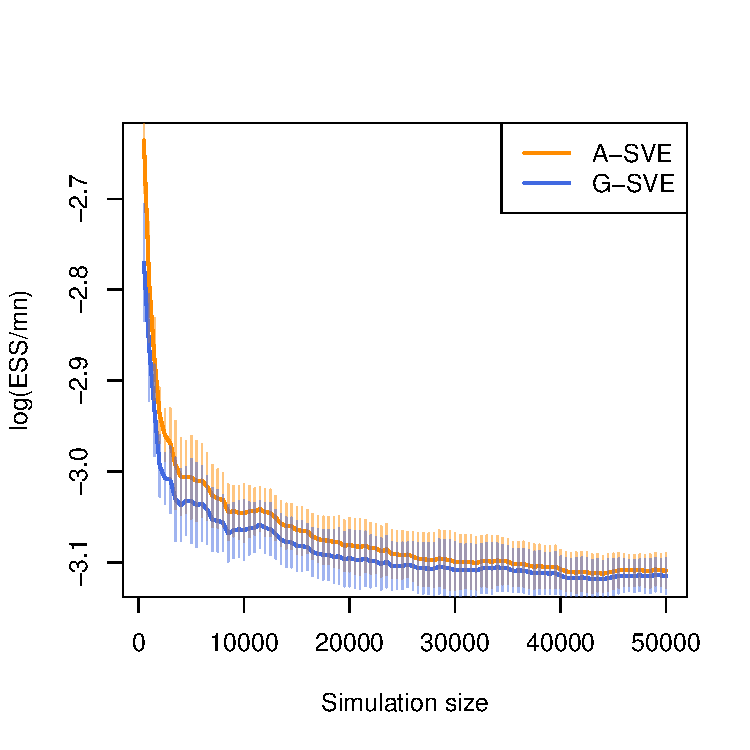
\includegraphics[width = .7\textwidth]{plots/boom-ess_1_10_7.pdf}
    \caption{Running plot for $\hat{ESS}/mn$ using ASV and RSV calculated for two chains (left) and five chains (right). The parameters of target distribution are $A = 1, \; B = 10, \; C = 7$}
    \label{fig:boom-ess_1_10_7}
\end{figure}

\begin{table}[h]
\centering
    \begin{tabular}{p{1cm}|p{2cm}|p{2cm}|p{2cm}|p{2cm}}
    \toprule
        n & \multicolumn{2}{|c|}{$m = 2$} & \multicolumn{2}{|c|}{$m=5$}\\
        \hline
        & ASV & RSV & ASV & RSV\\
        \hline
        $10^3$ & 0.873 & 0.884 & 0.875 & 0.898   \\
        $2\cdot10^3$ & 0.881 &  0.888 & 0.897    & 0.914     \\
        $5 \cdot 10^3$  & 0.902 & 0.908 &  0.919 & 0.929\\
        $10^4$  & 0.923 & 0.927 & 0.925 & 0.926 \\
        $5 \cdot 10^4$ & 0.951& 0.952 & 0.939 & 0.939  \\
    \bottomrule
    \end{tabular}
    \caption{Coverage probabilities for parameter values $A = 1,\; B = 10,\; C = 7$. }
    \label{table:boom-coverage_1_10_7}
\end{table}


\section{Discussion} \label{sec:discussion}


\appendix

\section{Preliminaries} \label{apdx:preliminaries}

\begin{lemma}
\label{lemma: brownian}
(\cite{csorgo2014strong}). Suppose Assumption \ref{ass:sip} holds, then for all $\epsilon > 0$ and for almost all sample paths, there exists $n_{0}\left(\epsilon\right)$ such that $\forall n\geq n_{0}$ and $\forall i = 1, ..., p$

\[
\sup_{0\leq t \leq n-b_n}\sup_{0 \leq s \leq b_n} \left| B^{\left(i\right)}\left(t+s\right) - B^{\left(i\right)}\left(t\right) \right| < \left(1+ \epsilon\right)\left(2b_n\left(\log\dfrac{n}{b_n} + \log\; \log\; n\right)\right)^{1/2} ,
\]

\[
\sup_{0 \leq s \leq b_n} \left|B^{\left(i\right)}\left(n\right) - B^{\left(i\right)}\left(n - s\right)\right| < \left(1+ \epsilon\right)\left(2b_n\left(\log\dfrac{n}{b_n} + \log\;\log\;n\right)\right)^{1/2} , \;and
\]

\[
\left|B^{\left(i\right)}\left(n\right)\right| < \left(1+\epsilon\right)\sqrt{2n\;\log \log n} \; . 
\]
\end{lemma}

\bigskip

\begin{lemma} \label{lemma:consis_1}
  Let the strong invariance principle hold. If $\dfrac{\psi(n)}{n} \to 0$ as $n \to \infty$, then $\|\overline\overline{{X}} - \mu\|_{\infty}, \|\overline{X}_s - \mu\|_{\infty} \xrightarrow[]{a.s.} 0$ as $n \to \infty$ for all $s \in \{1,..., m\}$\\
  \end{lemma}

\begin{proof}
Let $\|.\|$ denote the Euclidean norm. Assumption \ref{ass:sip} allows us to upper bound $\|\bar{X}_s - \mu\|_{\infty}$ using SIP. Following that, we show that the upper bound term converges to 0 as $n \to \infty$ using lemma \ref{lemma: brownian}.
 \begin{align*}
    \|\overline{X}_s - \mu\|_{\infty} & \leq \|\overline{X}_s - \mu\| \\
    &= \dfrac{1}{n}\left\|\sum_{t=1}^{n}X_{st} - n\mu\right\|\\
    &= \dfrac{1}{n}|\sum_{t=1}^{n}X_{st} - n\mu \pm L B(n)\|\\
    & \leq \dfrac{1}{n}\left\|\sum_{t=1}^{n}X_{st} - \mu - L B(n)\right\| + \dfrac{\left\|L B(n)\right\|}{n}\\
    &< \dfrac{D\psi(n)}{n} + \dfrac{\|L B(n)\|}{n}\\
    &< \dfrac{D\psi(n)}{n} + \dfrac{1}{n}\|L\| \left(\sum\limits_{i=1}^{p}|B^{(i)}(k)|^2\right)^{1/2}\\
    & \leq \dfrac{D\psi(n)}{n} + \dfrac{1}{n}\|L\| p^{1/2}(1+\epsilon)\sqrt{2n \log\log n}\\
    & \xrightarrow[]{a.s.} 0\;\; as \;\; n\to \infty
 \end{align*}

  Similarly one can easily show that $\|\bar{\bar{X}} - \mu\|_{\infty} \to 0$ as $n \to \infty$ using the same upper-bound as:
 
 \begin{align*}
    \|\overline{\overline{X}} - \mu\|_{\infty} & \leq \|\overline{\overline{X}} - \mu\|\\
    &= \dfrac{1}{m}\left\|\sum_{j=1}^{m}(\overline{X}_j- \mu) \right\|\\
    & \leq \dfrac{1}{m}\sum_{j=1}^{m}\|\overline{X}_j - \mu\|\\
    & \xrightarrow{a.s.} 0\qquad \textrm{as n} \to \infty 
\end{align*}
\end{proof}


\section{Proof of Theorems} \label{appendix:A}

\subsection{Strong consistency argument} \label{appendix:strong_consis}

\bigskip

\begin{lemma} \label{lemma:rsv_breakdown}
    The RSV estimator can be written as the sum of average pseudo SVE and two terms given by:
    \[
    \hat{\Sigma}_{RSV} = \tilde{\Sigma} + (1) + (2)
    \]
    where \\
    Term (1): $\dfrac{1}{m}\sum\limits_{s=1}^{m}\left\{\sum\limits_{k=-b_n+1}^{b_n-1}w_n\left(\dfrac{k}{b_n}\right)\sum\limits_{t=1}^{n-|k|}\dfrac{1}{n}\left[\left((X_{st}-\mu)_i(\mu-\overline{\overline{X}})_j\right)+ \left((\mu-\overline{\overline{X}})_i(X_{s(t+k)}-\mu)_j\right) \right]\right\}$\\
Term (2): $(\mu-\overline{\overline{X}})_i(\mu-\overline{\overline{X}})_j\sum\limits_{k=-b_n+1}^{b_n-1}\left(1-\dfrac{|k|}{n}\right)w_n\left(\dfrac{k}{n}\right)$
\end{lemma}

\begin{proof}
\begin{align*}
\hat{\Sigma}_{RSV}^{ij} &= \dfrac{1}{m}\sum_{s=1}^{m} \sum_{k=-b_n+1}^{b_n-1}w_n\left(\dfrac{k}{b_n}\right)\dfrac{1}{n}\sum_{t=1}^{n-|k|}(X_{st}-\overline{\overline{X}})_i(X_{s(t+k)}-\overline{\overline{X}})_j\\
&= \dfrac{1}{m}\sum_{s=1}^{m}\sum_{k=-b_n+1}^{b_n-1}w_n\left(\dfrac{k}{b_n}\right)\dfrac{1}{n}\sum_{t=1}^{n-|k|}[(X_{st}-\mu)_i+(\mu-\overline{\overline{X}})_i\}\{(X_{s(t+k)}-\mu)_j+(\mu-\overline{\overline{X}})_j]\\
&= \dfrac{1}{m}\sum_{s=1}^{m}\sum_{k=-b_n+1}^{b_n-1}w_n\left(\dfrac{k}{b_n}\right)\dfrac{1}{n}\sum_{t=1}^{n-|k|}[(X_{st}-\mu)_i(X_{s(t+k)}-\mu)_j+ (X_{st} - \mu)_i(\mu - \overline{\overline{X}})_j \\  & \; + (\mu-\overline{\overline{X}})_i(X_{s(t+k)}-\mu)_j+(\mu-\overline{\overline{X}})_i(\mu-\overline{\overline{X}})_j]\\
&= \tilde{\Sigma}^{ij} + \left[ \dfrac{1}{m}\sum_{s=1}^{m}\sum_{k=-b_n+1}^{b_n-1}w_n\left(\dfrac{k}{b_n}\right)\sum_{t=1}^{n-|k|}\left[\dfrac{1}{n}\left( (X_{st}-\mu)_i(\mu-\overline{\overline{X}})_j\right)+\dfrac{1}{n} \left((\mu-\overline{\overline{X}})_i(X_{s(t+k)}-\mu)_j\right) \right]\right] \\
& \; + \left[(\mu-\overline{\overline{X}})_i(\mu-\overline{\overline{X}})_j\sum_{k=-b_n+1}^{b_n-1}\left(1-\dfrac{|k|}{n}\right)w_n\left(\dfrac{k}{n}\right)\right]
\end{align*}

Therefore we get the following two terms:\\\\
Term (1): $\dfrac{1}{m}\sum\limits_{s=1}^{m}\left\{\sum\limits_{k=-b_n+1}^{b_n-1}w_n\left(\dfrac{k}{b_n}\right)\sum\limits_{t=1}^{n-|k|}\left[\dfrac{1}{n}\left((X_{st}-\mu)_i(\mu-\overline{\overline{X}})_j\right)+ \dfrac{1}{n}\left((\mu-\overline{\overline{X}})_i(X_{s(t+k)}-\mu)_j\right) \right]\right\}$\\
Term (2): $(\mu-\overline{\overline{X}})_i(\mu-\overline{\overline{X}})_j\sum\limits_{k=-b_n+1}^{b_n-1}\left(1-\dfrac{|k|}{n}\right)w_n\left(\dfrac{k}{n}\right)$\\
\\\\
\end{proof}

\bigskip

\begin{lemma} \label{lemma:pseudo_consis}
If the Assumption \ref{ass:sip}, \ref{ass:sve_consis} hold and $\dfrac{b_n \log \log n}{n} \to 0$, then $\tilde{\Sigma}^{ij} \xrightarrow{a.s.} \Sigma^{ij} \textrm{ as } n \to \infty$
\end{lemma}

\begin{proof}
We have,
\begin{align*}
    \tilde{\Sigma}^{ij} & = \dfrac{1}{m}\sum_{s=1}^{m}\sum_{k=-b_n+1}^{b_n-1}w_n\left(\dfrac{k}{b_n}\right)\dfrac{1}{n}\sum_{t=1}^{n-|k|}(X_{st}-\mu)_i(X_{s(t+|k|)} - \mu)_j\\
    & = \dfrac{1}{m}\sum_{s=1}^{m}\sum_{k=-b_n+1}^{b_n-1}w_n\left(\dfrac{k}{b_n}\right)\dfrac{1}{n}\sum_{t=1}^{n-|k|}(X_{st} \pm \overline{X}_s - \mu)_i(X_{s(t+|k|)} \pm \overline{X}_s - \mu)_j\\
    & = \hat{\Sigma}_{SV}^{ij} + \dfrac{1}{m}\sum_{s=1}^{m}\sum_{k=-b_n+1}^{b_n-1}w_n\left(\dfrac{k}{b_n}\right)\dfrac{1}{n}\sum_{t=1}^{n-|k|}\left[(X_{st} - \overline{X}_s)_i(\overline{X}_s - \mu)_j + (\overline{X}_s - \mu)_i(X_{s(t+k)} - \overline{X}_s)_j\right]\\
    & + \dfrac{1}{m}\sum_{s=1}^{m}(\overline{X}_s - \mu)_i(\overline{X}_s - \mu)_j\sum_{k=-b_n+1}^{b_n-1}w_n\left(\dfrac{k}{b_n}\right)\left(1 - \dfrac{\abs{k}}{b_n}\right)
\end{align*}
\\\\
Let Term (1*) be $\dfrac{1}{m}\sum\limits_{s=1}^{m}\sum\limits_{k=-b_n+1}^{b_n-1}w_n\left(\dfrac{k}{b_n}\right)\dfrac{1}{n}\sum\limits_{t=1}^{n-|k|}\left[(X_{st} - \overline{X}_s)_i(\overline{X}_s - \mu)_j + (\overline{X}_s - \mu)_i(X_{s(t+k)} - \overline{X}_s)_j\right]$
Let Term (2*) be $\dfrac{1}{m}\sum\limits_{s=1}^{m}(\overline{X}_s - \mu)_i(\overline{X}_s - \mu)_j\sum\limits_{k=-b_n+1}^{b_n-1}w_n\left(\dfrac{k}{b_n}\right)\left(1 - \dfrac{\abs{k}}{b_n}\right)$
\\\\
We will prove that Term (1*), Term (2*) $\xrightarrow{a.s.} 0 \textrm{ as } n \to \infty$. From \cite{vats:fleg:jon:2018}, we have that $\hat{\Sigma}_{SV} \to 0$ with probability 1 as $n \to \infty$ for multivariate case. Assuming that all the assumptions made there hold true for our case, we will prove that $\tilde{\Sigma} \to 0$ with probability 1 as $n \to \infty$. 
\\\\

Firstly, we prove that Term (1*) $\xrightarrow{a.s.} 0$ as $n \to \infty$. We will prove this for the first part of Term (1*). It will hold true equivalently for the second part as well. The first part of the Term (1*) is,


\begin{align*}
    & \dfrac{1}{m}\sum\limits_{s=1}^{m}\sum\limits_{k=-b_n+1}^{b_n-1}w_n\left(\dfrac{k}{b_n}\right)\dfrac{1}{n}\sum\limits_{t=1}^{n-|k|}\left[(X_{st} - \overline{X}_s)_i(\overline{X}_s - \mu)_j \right]\\
    & = \dfrac{1}{m}\sum\limits_{s=1}^{m}\sum\limits_{k=-b_n+1}^{b_n-1}w_n\left(\dfrac{k}{b_n}\right)\dfrac{(\bar{X}_s - \mu)_j}{n}\left[\sum\limits_{t=1}^{|k|}(\overline{X}_s - X_{st})_i\right]\\
    & = \dfrac{1}{m}\sum\limits_{s=1}^{m}\sum\limits_{k=-b_n+1}^{b_n-1}w_n\left(\dfrac{k}{b_n}\right)\dfrac{(\bar{X}_s - \mu)_j}{n}\left[\sum\limits_{t=1}^{|k|}(\mu - X_{st})_i + \abs{k}(\overline{X}_s - \mu)_i\right]\\
    & \leq \dfrac{1}{m}\sum\limits_{s=1}^{m}\sum\limits_{k=-b_n+1}^{b_n-1}w_n\left(\dfrac{k}{b_n}\right)\dfrac{\|\bar{X}_s - \mu\|_{\infty}}{n}\left\|\sum\limits_{t=1}^{|k|}(\mu - X_{st}) + \abs{k}\overline{X}_s - \mu)\right\|_{\infty}\\
    & \leq \dfrac{1}{m}\sum\limits_{s=1}^{m}\sum\limits_{k=-b_n+1}^{b_n-1}w_n\left(\dfrac{k}{b_n}\right)\dfrac{\|\bar{X}_s - \mu\|_{\infty}}{n}\left(\left\|\sum\limits_{t=1}^{|k|}(X_{st} - \mu)\right\|_{\infty} + \abs{k}\|\overline{X}_s - \mu\|_{\infty} \right)\\
    & \leq \dfrac{1}{m}\sum\limits_{s=1}^{m}\sum\limits_{k=-b_n+1}^{b_n-1}\dfrac{\|\bar{X}_s - \mu\|_{\infty}}{n}\left\|\sum\limits_{t=1}^{|k|}(\overline{X}_s - \mu)\right\| + \dfrac{1}{m}\sum\limits_{s=1}^{m} \dfrac{b_n(b_n-1)}{n}\|\bar{X}_s - \mu\|_{\infty}^2
\end{align*}

Using SIP on the summation of k terms,
\begin{multline*}
    & < \dfrac{1}{m}\sum\limits_{s=1}^{m}\|\bar{X}_s - \mu\|_{\infty}\sum\limits_{k=-b_n + 1}^{b_n-1}\left[ \dfrac{D \psi(k)}{n} + \dfrac{\|L\| p^{1/2}(1+\epsilon)\sqrt{2k \log\log k}}{n}  \right] + \dfrac{1}{m}\sum\limits_{s=1}^{m} \dfrac{b_n(b_n-1)}{n}\|\bar{X}_s - \mu\|_{\infty}^2\\
    & < \dfrac{(2b_n-1)}{m}\sum\limits_{s=1}^{m}\|\bar{X}_s - \mu\|_{\infty}\left[ \dfrac{D \psi(n)}{n} + \dfrac{\|L\| p^{1/2}(1+\epsilon)\sqrt{2n \log\log n}}{n}  \right] + \dfrac{1}{m}\sum\limits_{s=1}^{m} \dfrac{b_n(b_n-1)}{n}\|\bar{X}_s - \mu\|_{\infty}^2
\end{multline*}

Using lemma \ref{lemma:consis_1}, the above term can be upper bounded by,

\begin{equation} \label{eq:PASVE_term-1}
  \left(2b_n - 1 + \dfrac{b_n^2}{n} + \dfrac{b_n}{n}\right)\left[ \dfrac{D \psi(n)}{n} + \dfrac{\|L\| p^{1/2}(1+\epsilon)\sqrt{2n \log\log n}}{n}  \right]^2  
\end{equation}
\\
Using the bound on $\psi(n)$ given by \cite{stra:1964}, (\ref{eq:PASVE_term-1}) becomes $\mathcal{O}\left(b_n \log \log n/n\right)$ which converges to 0 as $n \to \infty$.
\\
Similar to the above proof, second part of Term (1*) can also be written as a summation of k terms and the proof follows exactly as the first part. Now we prove that Term (2*) $\xrightarrow{a.s.} 0 \textrm{ as } n \to \infty$.

\begin{align*}
    &\dfrac{1}{m}\sum\limits_{s=1}^{m}(\overline{X}_s - \mu)_i(\overline{X}_s - \mu)_j\sum\limits_{k=-b_n+1}^{b_n-1}w_n\left(\dfrac{k}{b_n}\right)\left(1 - \dfrac{\abs{k}}{b_n}\right)\\
    & < \dfrac{1}{m}\sum\limits_{s=1}^{m} \|\overline{X}_s - \mu\|_{\infty}^2 \sum\limits_{k=-b_n+1}^{b_n-1}\left|w_n\left(\dfrac{k}{b_n}\right)\right|\\
    & = \dfrac{b_n}{m}\sum\limits_{s=1}^{m} \|\overline{X}_s - \mu\|_{\infty}^2 \dfrac{1}{b_n} \sum\limits_{k=-b_n+1}^{b_n-1}\left|w_n\left(\dfrac{k}{b_n}\right)\right|\\
    & \leq \dfrac{b_n}{m}\sum\limits_{s=1}^{m} \|\overline{X}_s - \mu\|_{\infty}^2 \int_{-\infty}^{\infty} \abs{w_n(x)}dx
\end{align*}
\\
Recall that the lag window is such that $\int_{-\infty}^{\infty} \abs{w_n(x)}dx = C$ for some constant C. Using lemma \ref{lemma:consis_1}, Term (2*) can be upper bounded by

\begin{equation} \label{eq:PASVE_term-2}
    Cb_n\left[ \dfrac{D \psi(n)}{n} + \dfrac{\|L\| p^{1/2}(1+\epsilon)\sqrt{2n \log\log n}}{n}  \right]^2 
\end{equation}

(\ref{eq:PASVE_term-2}) is also $\mathcal{O}\left(\dfrac{b_n \log \log n}{n}\right)$, and hence converges to 0 as $n \to \infty$.

\end{proof}



\bigskip


\begin{proof}[Proof of theorem \ref{th:consistency}]
We first show that Term (1) $\xrightarrow{a.s} 0$ as $n \to \infty$ with the help of SIP and prior assumptions.
\begin{align*}
   & \left|\dfrac{1}{m}\sum\limits_{s=1}^{m}\left\{\sum\limits_{k=-b_n+1}^{b_n-1}w_n\left(\dfrac{k}{b_n}\right)\sum\limits_{t=1}^{n-|k|} \dfrac{1}{n}\left[(X_{st}-\mu)_i(\mu-\overline{\overline{X}})_j+ (\mu-\overline{\overline{X}})_i(X_{s(t+k)}-\mu)_j\right]\right\}\right| \\
   & \leq \dfrac{1}{m}\sum\limits_{s=1}^{m}\left\{\sum\limits_{k=-b_n+1}^{b_n-1}w_n\left(\dfrac{k}{b_n}\right)\left[ \dfrac{1}{n}{\left|\sum\limits_{t=1}^{n-|k|}(X_{st}-\mu)_i(\mu-\overline{\overline{X}})_j\right|}+\dfrac{1}{n}{\left|\sum\limits_{t=1}^{n-|k|}(\mu-\overline{\overline{X}})_i(X_{s(t+k)}-\mu)_j\right|} \right]\right\}
\end{align*}

\begin{align*}
    & \leq \dfrac{1}{m}\sum\limits_{s=1}^{m}\left\{\sum\limits_{k=-b_n+1}^{b_n-1}w_n\left(\dfrac{k}{b_n}\right)\left[ \dfrac{1}{n}\left|\sum\limits_{t=1}^{n-|k|}(X_{st}- \mu)_i\right|\left|(\mu-\overline{\overline{X}})_j\right|+ \dfrac{1}{n}\left|(\mu-\overline{\overline{X}})_i\right|\left|\sum\limits_{t=1}^{n-|k|}(X_{j(t+k)}-\mu)_j\right|\right]\right\}\\
    & \leq \dfrac{\|(\overline{\overline{X}} - \mu)\|_{\infty}}{m}\sum\limits_{s=1}^{m}\sum\limits_{k=-b_n+1}^{b_n-1}\left[ \dfrac{1}{n}\left\|\sum\limits_{t=1}^{n-|k|}(X_{st}-\mu)\right\|_{\infty} + \dfrac{1}{n}\left\|\sum\limits_{t=1}^{n-|k|}(X_{s(t+k)}-\mu)\right\|_{\infty} \right]\\
    &\leq \dfrac{\|(\overline{\overline{X}} - \mu)\|_{\infty}}{m} \sum\limits_{s=1}^{m}\sum\limits_{k=-b_n+1}^{b_n-1}\left[ \dfrac{1}{n}\left\|\sum\limits_{t=n-|k|+1}^{n}(X_{st} - \mu) - n(\overline{X}_s - \mu) \right\|_{\infty} + \dfrac{1}{n}\left\|\sum\limits_{t=1}^{|k|}(X_{st} - \mu) - n(\overline{X}_s - \mu)\right\|_{\infty} \right]\\
    &\leq \dfrac{\|(\overline{\overline{X}} - \mu)\|_{\infty}}{m} \sum\limits_{s=1}^{m}\sum\limits_{k=-b_n+1}^{b_n-1}\left[ \dfrac{1}{n}\left\|\sum\limits_{t=n-|k|+1}^{n}(X_{st} - \mu)\right\|_{\infty} + \dfrac{1}{n}\left\|\sum\limits_{t=1}^{|k|}(X_{st} - \mu)\right\|_{\infty} + 2\|\overline{X}_s - \mu\|_{\infty} \right]\\
    & \leq \dfrac{\|(\overline{\overline{X}} - \mu)\|_{\infty}}{m} \sum\limits_{s=1}^{m}\sum\limits_{k=-b_n + 1}^{b_n-1}\left[ \dfrac{1}{n}\left\|\sum\limits_{t=n-|k|+1}^{n}(X_{st} - \mu)\right\| + \dfrac{1}{n}\left\|\sum\limits_{t=1}^{|k|}(X_{st} - \mu)\right\| \right]\\
    & \; \;+ 2(2b_n - 1)\|\overline{\overline{X}} - \mu\|_{\infty}\|\overline{X}_1 - \mu\|_{\infty} 
\end{align*}
\\
Using SIP on summation of $k$ terms, we obtain the following upper bound for Term (1)
\begin{align*}
    & < 2\|(\overline{\overline{X}} - \mu)\|_{\infty}\sum\limits_{k=-b_n + 1}^{b_n-1}\left[ \dfrac{D \psi(k)}{n} + \dfrac{\|L\| p^{1/2}(1+\epsilon)\sqrt{2k \log\log k}}{n}  \right] + 2(2b_n - 1)\|\overline{\overline{X}} - \mu\|_{\infty}\|\overline{X}_1 - \mu\|_{\infty} \\
    &\leq 2(2b_n - 1)\|(\overline{\overline{X}} - \mu)\|_{\infty} \left[ \dfrac{D \psi(n)}{n} + \dfrac{\|L\| p^{1/2}(1+\epsilon)\sqrt{n \log\log n}}{n}  \right] + 2(2b_n - 1)\|\overline{\overline{X}} - \mu\|_{\infty}\|\overline{X}_1 - \mu\|_{\infty}
\end{align*}
\\
We use lemma \ref{lemma:consis_1} to upper bound the above term as
\begin{equation} \label{eq:strong_consis_term-1}
    4(2b_n - 1)\left[ \dfrac{D \psi(n)}{n} + \dfrac{\|L\| p^{1/2}(1+\epsilon)\sqrt{n \log\log n}}{n}  \right]^2
\end{equation}
\\
Using the bound on $\psi(n)$ given by \cite{stra:1964}, equation (\ref{eq:strong_consis_term-1}) becomes $\mathcal{O}\left(b_n \log \log n/n\right)$ which converges to 0 as $n \to \infty$. Now we will show that Term (2) $\xrightarrow{a.s.} 0$ as $n\to \infty$

\begin{align*}
    &\left|\dfrac{1}{m}\sum\limits_{s=1}^{m}\left\{(\mu-\overline{\overline{X}})_i(\mu-\overline{\overline{X}})_j\sum_{k=-b_n+1}^{b_n-1}\left(1-\dfrac{|k|}{n}\right)w_n\left(\dfrac{k}{n}\right)\right\}\right|\\
    & \leq\|\overline{\overline{X}} - \mu\|_{\infty}^2\left[\sum_{k=-b_n+1}^{b_n-1}\left(1-\dfrac{|k|}{n}\right)w_n\left(\dfrac{k}{n}\right)\right]\\
    &< \|\overline{\overline{X}} - \mu\|_{\infty}^2\left[\sum_{k=-b_n+1}^{b_n-1}\left|w_n\left(\dfrac{k}{n}\right)\right|\right]\\
    &= b_n\|\overline{\overline{X}} - \mu\|_{\infty}^2\left[\dfrac{1}{b_n}\sum_{k=-b_n+1}^{b_n-1}\left|w_n\left(\dfrac{k}{n}\right)\right|\right]\\
    & \leq b_n\|\overline{\overline{X}} - \mu\|_{\infty}^2 \int_{-\infty}^{\infty}|w_n(x)|dx \\
    & \leq Cb_n\|\overline{\overline{X}} - \mu \|^2
\end{align*}

Using lemma \ref{lemma:consis_1} to upper bound the above term as 

\begin{equation} \label{eq:strong_consis_term-2}
     Cb_n\left[ \dfrac{D \psi(n)}{n} + \dfrac{\|L\| p^{1/2}(1+\epsilon)\sqrt{n \log\log n}}{n}  \right]^2
\end{equation}
\\
Equation (\ref{eq:strong_consis_term-2}) has the same order as equation (\ref{eq:strong_consis_term-1}), i.e. $\mathcal{O}\left(b_n \log \log n/n\right) \to 0 \textrm{ as } n \to \infty$.
We have already shown that Term (1) and Term (2) converge to 0 almost surely $\implies \hat{\Sigma}_{RSV} \xrightarrow{a.s.} \tilde{\Sigma}$ as $n \to \infty$. Now we can find the functions $g_1(n), g_2(n) \textrm{ and, } g_3(n)$ by adding (\ref{eq:strong_consis_term-1}) and (\ref{eq:strong_consis_term-2}). After some simple algebra, we obtain the following results:\\

\begin{align*}
    g_1(n) &= (4+C_1)\dfrac{b_n \psi^2(n)}{n^2} - 4\dfrac{\psi^2(n)}{n^2} \to 0\\
    g_2(n) &= 2\sqrt{2}\|L\|p^{1/2}(1+\epsilon)\left[(4+C_1)\dfrac{b_n\psi(n)\sqrt{n\log \log n}}{n^2} - 4\dfrac{\psi(n)\sqrt{n\log \log n}}{n^2}\right] \to 0\\
    g_3(n) &= \|L\|^2 p (1+\epsilon)^2\left[(4+C_1)\dfrac{b_n \log\log n}{n} - 4 \dfrac{\log \log n}{n}\right] \to 0
\end{align*}
\end{proof}

\\
\subsection{Bias Calculations} \label{appendix:bias}

 
\begin{lemma} \label{lemma:bias1}
$\mathbb{E}[(X_{11}-\overline{X}_1)(\overline{X}_1 - \overline{\overline{X}})^T] = \dfrac{m-1}{mn}\left(\sum\limits_{k=0}^{n-1}\Gamma(k) - \Sigma\right)$
\end{lemma}
\begin{proof}
\begin{align*}
    &\mathbb{E}[(X_{11}-\overline{X}_1)(\overline{X}_1 - \overline{\overline{X}})^T] = \mathbb{E}[X_{11}\overline{X}_1^T] - \mathbb{E}[X_{11}\overline{\overline{X}}^T] + \mathbb{E}[\overline{X}_1\overline{\overline{X}}^T] - \mathbb{E}[\overline{X}_1\overline{X}_1^T]\\
    &= \mathbb{E}[X_{11}\overline{X}_1^T] - \dfrac{1}{m}\mathbb{E}[X_{11}\overline{X}_1^T] - \dfrac{m-1}{m}\mathbb{E}[X_{11}\overline{X}_2^T] + \dfrac{1}{m}\mathbb{E}[\overline{X}_1\overline{X}_1^T] + \dfrac{m-1}{m}\mathbb{E}[\overline{X}_1\overline{X}_2^T] - \mathbb{E}[\overline{X}_1\overline{X}_1^T]\\
    &= \dfrac{m-1}{m}\left(\mathbb{E}[X_{11}\overline{X}_1^T] - \mathbb{E}[X_{11}\overline{X}_2^T] + \mathbb{E}[\overline{X}_1\overline{X}_2^T] - \mathbb{E}[\overline{X}_1\overline{X}_1^T]\right)\\
    &= \dfrac{m-1}{m}\left(\dfrac{1}{n}\sum_{i=1}^{n}\mathbb{E}[X_{11}X_{1i}^T] - \mathbb{E}[X_{11}]\mathbb{E}[\overline{X}_2^T] + \mathbb{E}[\overline{X}_1]\mathbb{E}[\overline{X}_2^T] - Var[\overline{X}_1] - \mathbb{E}[\overline{X}_1]\mathbb{E}[\overline{X}_1^T]\right)\\
    &= \dfrac{m-1}{m}\left(\dfrac{1}{n}\sum_{k=0}^{n-1}\Gamma(k) + \mu \mu^T - \mu \mu^T + \mu \mu^T - \dfrac{\Sigma}{n} - \mu \mu^T\right)\\
    &= \dfrac{m-1}{mn}\left(\sum_{k=0}^{n-1}\Gamma(k) - \Sigma\right)
\end{align*}
\\   
Similarly, we can show that $\mathbb{E}[A_{ij}^T] = \mathbb{E}[A_{ij}]$ using the symmetry of $\Gamma(k) \textrm{ and } \Sigma$ matrices.
    
\begin{align*}
    \mathbb{E}[(\bar{X}_1 - \bar{\bar{X}})(X_{11}-\bar{X}_1)^T] &= \mathbb{E}[(X_{11}-\bar{X}_1)(\bar{X}_1 - \bar{\bar{X}})^T]^T\\
    &= \dfrac{m-1}{mn}\left(\sum_{k=0}^{n-1}\Gamma(k) - \Sigma \right)^T\\
    &= \dfrac{m-1}{mn}\left(\sum_{k=0}^{n-1}\Gamma(k) - \Sigma \right)\\
\end{align*}
\end{proof}


\begin{lemma} \label{lemma:bias2}
$$\mathbb{E}\left[\sum\limits_{s=1}^{m}(\overline{X}_{s}-\overline{\overline{X}})(\overline{X}_{s}-\overline{\overline{X}})^{T}\right] =  (m-1)\Var(\overline{X_1})$$
\end{lemma}
\\
$\overline{X}_i$ are independently and identically distributed for all $i$; this implies $\Var(\overline{\overline{X}}) = \dfrac{1}{m} \Var(\overline{X}_1)$. 

\begin{proof}
\begin{align*}
\mathbb{E}\left[\sum\limits_{s=1}^{m}(\overline{X}_{s}-\overline{\overline{X}})(\overline{X}_{s}-\overline{\overline{X}})^{T}\right] &= \mathbb{E}\left[\sum_{s=1}^{m}\overline{X}_{s}\overline{X}_{s}^{T} -\sum_{s=1}^{m}\overline{X}_{s}\overline{\overline{X}}^{T} - \overline{\overline{X}}^{T}\sum_{s=1}^{m}\overline{X}_{s}^{T} + m\overline{\overline{X}}\overline{\overline{X}}^{T}\right]\\
&= \mathbb{E}\left[\sum_{s=1}^{m}\overline{X}_{s}\overline{X}_{s}^{T} - m\overline{\overline{X}}\overline{\overline{X}}^{T}\right]\\
&= m\left(\mathbb{E}\left[\overline{X}_{1}\overline{X}_{1}^{T}\right] - \mathbb{E}\left[\overline{\overline{X}}\overline{\overline{X}}^{T}\right]\right)\\
&= m\left(Var(\overline{X}_{1}) + \mu\mu^{T} - Var(\overline{\overline{X}}) - \mu\mu^{T}\right)\\
&= (m-1)\Var(\overline{X_1})
\end{align*}
\end{proof}


\begin{proof}[Proof of theorem \ref{th:RAC_expec}]
\begin{align*}
    \hat{\Gamma}_{RAC}(k) &= \dfrac{1}{m}\sum_{s=1}^{m}\hat{\Gamma}_{RAC,s}(k) = \dfrac{1}{mn}\sum_{s=1}^{m}\sum_{t=1}^{n-|k|}(X_{st}-\overline{\overline{X}})(X_{s(t+k)}-\overline{\overline{X}})^T\\
    &= \left[\dfrac{1}{mn}\sum_{s=1}^{m}\sum_{t=1}^{n-|k|}(X_{st}-\overline{X_s})(X_{s(t+k)}-\overline{X_s})^T\right] + \left[\dfrac{1}{mn}\sum_{s=1}^{m}\sum_{t=1}^{|k|}(\overline{X}_s - \overline{\overline{X}})(\overline{X}_s - X_{st})^T\right]\\ 
    &+  \left[\dfrac{1}{mn}\sum_{s=1}^{m}\sum_{t=n-|k|+1}^{n}( \overline{X}_s - X_{st})(\overline{X_s}-\overline{\overline{X}})^T\right] + \left[\dfrac{n-|k|}{mn}\sum_{s=1}^{m}(\overline{X_s}-\overline{\overline{X}})(\overline{X_s}-\overline{\overline{X}})^T\right]\\
    &= \dfrac{1}{m}\sum_{s=1}^{m}\hat{\Gamma}_s(k) - \dfrac{1}{mn}\sum_{s=1}^{m}\sum_{t=1}^{|k|}A_{st}^T - \dfrac{1}{mn}\sum_{s=1}^{m}\sum_{t=n-|k|+1}^{n}A_{st} + \dfrac{n-|k|}{mn}\sum_{s=1}^{m}(\overline{X_s}-\overline{\overline{X}})(\overline{X_s}-\overline{\overline{X}})^T
\end{align*}

where $A_{st} = (X_{st}-\overline{X}_s)(\overline{X}_s - \overline{\overline{X}})^T$.\\


\\
Using equation \ref{eq:priestly}, lemma \ref{lemma:bias1}, and lemma \ref{lemma:bias2}, the expectation of $\hat{\Gamma}_{RAC}(k)$ can be written as 

\begin{align*}
    &= \left(1- \dfrac{|k|}{n}\right)\left(\Gamma(k) - \Var(\overline{X_1})\right) - \dfrac{1}{n} \left(\sum\limits_{t=1}^{|k|}\mathbb{E}[A_{1t}^T] + \sum\limits_{t=n-|k|+1}^{n}\mathbb{E}[A_{1t}]\right) + \left(1- \dfrac{|k|}{n}\right)\left(1-\dfrac{1}{m}\right)\Var(\overline{X_1})\\
    &= \left(1- \dfrac{|k|}{n}\right)\left(\Gamma(k) - \dfrac{1}{m}\Var(\overline{X_1})\right) - \dfrac{2|k|}{n}\dfrac{m-1}{mn}\left(\sum_{h=0}^{n-1}\Gamma(h) - \Sigma\right)
\end{align*}
\\
Using the results of \cite{song1995optimal} given in equation \ref{eq:song} to expand $\Var(\overline{X}_1)$,
\[
\mathbb{E}[\hat{\Gamma}_{RAC}(k)] = \left(1- \dfrac{|k|}{n}\right)\left(\Gamma(k) - \dfrac{\Sigma}{mn} - \dfrac{\Phi}{mn^2}\right)  + \dfrac{2(m-1)}{m}\dfrac{\abs{k}}{n^2} \left(\Sigma - \sum_{h=0}^{n-1}\Gamma(h)\right) + o(n^{-2})
\]
\\
We observe that this expectation result is very similar to equation \ref{eq:priestly} from \cite{priestley1981spectral} for the asymptotically unbiased estimator of autocovariance except for an additional positive bias term. This helps in countering the inherent negative bias in $\hat{\Gamma}(k)$ and give more informative estimates of autocovariance.  Although, bias term for a fixed $k$ is $o(1)$, it increases with $k$. We have explicitly written the end effect term arising from using the estimator $\overline{\overline{X}}$ for $\mu$. These are small order terms that vanish as $n \to \infty$.
\end{proof}

\begin{proof}[Proof of corollary \ref{cor:lag0_expectation}]

\begin{align*}
    \hat{\Gamma}_{RAC}(k) &= \dfrac{1}{m}\sum_{s=1}^{m}\hat{\Gamma}_{RAC,s}(k) = \dfrac{1}{mn}\sum_{s=1}^{m}\sum_{t=1}^{n}(X_{st}-\overline{\overline{X}})(X_{s(t+k)}-\overline{\overline{X}})^T\\
    &= \left[\dfrac{1}{mn}\sum_{s=1}^{m}\sum_{t=1}^{n}(X_{st}-\overline{X_s})(X_{s(t+k)}-\overline{X_s})^T\right] + \left[\dfrac{1}{m}\sum_{s=1}^{m}(\overline{X_s}-\overline{\overline{X}})(\overline{X_s}-\overline{\overline{X}})^T\right]\\
    &= \dfrac{1}{m}\sum_{s=1}^{m}\hat{\Gamma}_s(k)  + \dfrac{1}{m}\sum_{s=1}^{m}(\overline{X_s}-\overline{\overline{X}})(\overline{X_s}-\overline{\overline{X}})^T
\end{align*}
Using equation \ref{eq:priestly}, lemma \ref{lemma:bias2}, and equation \ref{eq:song} the expectation of $\hat{\Gamma}_{RAC}(0)$ can be written as 

\begin{align*}
    \mathbb{E}[\hat{\Gamma}_{RAC}(0)] &= \left(\Gamma(k) - \Var(\overline{X_1})\right) + \left(1-\dfrac{1}{m}\right)\Var(\overline{X_1})\\
    &= \Gamma(k) - \dfrac{1}{m}\Var(\overline{X_1})\\
    &= \Gamma(0) - \dfrac{\Sigma}{mn} - \dfrac{\Phi}{mn^2} + o(n^{-2})
\end{align*}

\end{proof}


\begin{proof}[Proof of theorem \ref{th:rsv_bias}]
The convoluted end effect terms in theorem \ref{th:RAC_expec} are all essentially $\mathcal{O}(1/n)$. We are interested in finding the asymptotic bias here. Therefore we can write the expection of replicated autocovariance as 
\begin{equation} \label{eq:rac_bias2}
\mathbb{E}[\hat{\Gamma}_{RAC}(k)] = \left(1 - \dfrac{\abs{k}}{n}\right)\Gamma(k) + \left(1 - \dfrac{\abs{k}}{n}\right)\mathcal{O}(1/n) + \mathcal{O}(1/n)    
\end{equation}

The last term in (\ref{eq:rac_bias2}) is stated separately because it does not depend on $k$. 
\begin{align*}
    &\mathbb{E}[\hat{\Sigma}_{RSV} - \Sigma]\\
    &= \sum_{k=-b_n+1}^{b_n-1} w\left(\dfrac{|k|}{b_n}\right)\mathbb{E}[\hat{\Gamma}_{RAC}(k)]-\sum_{k=-\infty}^{\infty}\Gamma(k)\\
    &= \sum_{k=-b_n+1}^{b_n-1}\left\{ w_n\left(\dfrac{|k|}{b_n}\right)\left(1-\dfrac{|k|}{n}\right)\left[\left(\Gamma(k) + \mathcal{O}\left(\dfrac{1}{n}\right)\right) + \mathcal{O}\left(\dfrac{1}{n}\right)\right]\right\} - \sum_{k=-\infty}^{\infty}\Gamma(k)\\
    &= \sum_{k=-b_n+1}^{b_n-1}\left\{ w_n\left(\dfrac{|k|}{b_n}\right)\left(1-\dfrac{|k|}{n}\right)\Gamma(k) \right\} - \sum_{k=-\infty}^{\infty}\Gamma(k)\\
    &+ \sum_{k=-b_n+1}^{b_n-1}\left\{ w_n\left(\dfrac{|k|}{b_n}\right)\left[\left(1-\dfrac{|k|}{n}\right)\mathcal{O}\left(\dfrac{1}{n}\right) + \mathcal{O}\left(\dfrac{1}{n}\right)\right] \right\}
\end{align*}
Since $w_n\left(\dfrac{k}{b_n}\right) = 0$ for $|k| > b_n$, we can decompose the above term as:\\
Let Term \textbf{A}: $\sum\limits_{k=-n+1}^{n-1}\left\{w_n\left(\dfrac{|k|}{b_n}\right)\left(1-\dfrac{|k|}{n}\right)\Gamma(k) \right\} - \sum\limits_{k=-\infty}^{\infty}\Gamma(k)$\\ 

Let Term \textbf{B}: $\sum\limits_{k=-n+1}^{n-1}\left\{w\left(\dfrac{|k|}{b_n}\right)\left[\left(1-\dfrac{|k|}{n}\right)\mathcal{O}\left(\dfrac{1}{n}\right) + \mathcal{O}\left(\dfrac{1}{n}\right)\right] \right\}$\\\\

\begin{enumerate}
    \item We first solve for term {\textbf{A}} by breaking it into three parts as in \cite{hannan2009multiple}.\\

$$-\sum_{|k|\geq n}\Gamma(k) + \sum_{k = -n+1}^{n-1}w_n\left(\dfrac{|k|}{n}\right)\dfrac{|k|}{n}\Gamma(k)- \sum_{k = -n+1}^{n-1}\left(1-w_n\left(\dfrac{|k|}{n}\right)\right)\Gamma(k)$$\\

We deal with the three subterms of term \textbf{A} individually,
\begin{enumerate}
    \item 
    \begin{align*}
        \left\|{-\sum_{|k|\geq n}\Gamma(k)}\right\| &\leq   \abs{\dfrac{k}{n}}^q\sum_{|k|\geq n}\|\Gamma(k)\|\\
        &= \dfrac{1}{b_n^q}\abs{\dfrac{b_n}{n}}^q\underbrace{\sum_{|k|\geq n}|k|^q\|\Gamma(k)\|}_{<\infty}\\
        &= o\left(\dfrac{1}{b_n^q}\right)
    \end{align*}
    
    \item
\begin{align*}
   \left\| \sum_{k = -n+1}^{n-1}w_n\left(\dfrac{|k|}{n}\right)\dfrac{|k|}{n}\Gamma(k)\right\| &\leq \dfrac{c}{n}\sum_{k = -n+1}^{n-1}|k|\|\Gamma(k)\| 
\end{align*}
 
 \begin{enumerate}
     \item For q $\geq 1$, we have, $\sum_{k=-n+1}^{n-1}|k|^q\|\Gamma(k)\| < \infty$
     \begin{align*}
         \dfrac{c}{n}\sum_{k = -n+1}^{n-1}|k|\|\Gamma(k)\| &\leq \dfrac{c}{n}\sum_{k = -n+1}^{n-1}|k|^q\|\Gamma(k)\|\\
         &= \dfrac{1}{b_n^q}\dfrac{b_n^q}{n}c\sum_{k = -n+1}^{n-1}|k|^q\|\Gamma(k)\|\\
         &= o\left(\dfrac{1}{b_n^q}\right) 
     \end{align*}
     
     
     \item For q $<1$:\\
     \begin{align*}
         c\sum_{k =-n+1}^{n-1}\dfrac{|k|}{n}\|\Gamma(k)\| &\leq c\sum_{k =-n+1}^{n-1}\abs{\dfrac{k}{n}}^q\|\Gamma(k)\|\\
         &= \dfrac{1}{b_n^q}\dfrac{b_n^q}{n}c\sum_{k =-n+1}^{n-1}|k|^q\|\Gamma(k)\|\\
         &= o\left(\dfrac{1}{b_n^q}\right) 
     \end{align*}
     \end{enumerate}
     \item 
     $$\sum_{k = -n+1}^{n-1}\left(1-w_n\left(\dfrac{|k|}{b_n}\right)\right)\Gamma(k) = -\dfrac{1}{b_n^q}\sum_{k = -n+1}^{n-1}\left[\dfrac{\left(1-w_n\left(\dfrac{|k|}{b_n}\right)\right)}{\left(\dfrac{|k|}{b_n}\right)^q}|k|^q \Gamma(k)\right]$$\\
     
     The condition 
     \[
     \lim_{\abs{x}\to 0}\dfrac{1 - w_n(x)}{\abs{x}^q} = k_q < \infty
     \]
     implies that $\dfrac{1-w_n(k/b_n)}{\abs{k/b_n}^q}$ converges boundedly to $k_q$ for each $k$; where $k_q$ is specific to the lag-window used. Taking the limiting value, we have
     \[
     \lim_{n \to \infty}\sum_{k = -n+1}^{n-1}\left(1-w_n\left(\dfrac{|k|}{b_n}\right)\right)\Gamma(k) = -\dfrac{k_q \Phi^{(q)}}{b_n^q}
     \]
\end{enumerate}

 \item Solving for Term \circled{\textbf{B}}. We will find an upper bound and prove that it is $\mathcal{O}\left(\dfrac{1}{n}\right)$:
 \begin{align*}
     & \sum_{k=-n+1}^{n-1}\left\{w_n\left(\dfrac{|k|}{b_n}\right)\left[\left(1-\dfrac{|k|}{n}\right)\mathcal{O}\left(\dfrac{1}{n}\right) + \mathcal{O}\left(\dfrac{1}{n}\right) \right] \right\} \\
     &\leq \sum_{k=-n+1}^{n-1}w_n\left(\dfrac{|k|}{b_n}\right)\mathcal{O}\left(\dfrac{1}{n}\right)\\
     &= \mathcal{O}\left(\dfrac{1}{n}\right) \sum_{k=-n+1}^{n-1}w_n\left(\dfrac{|k|}{b_n}\right) \\
     &= \mathcal{O}\left(\dfrac{1}{n}\right) 2\pi W_n \\
     &= \mathcal{O}\left(\dfrac{1}{n}\right) \\
     &= o\left(\dfrac{1}{b_n^q}\right) 
 \end{align*}
 \end{enumerate}  
 \\
 We have shown that all, but one, terms are $o(1/b_n^q)$. Therefore, the limiting value of $b_n^q\mathbb{E}[\hat{\Sigma}_{RAC} - \Sigma]$ is proved to be same as that of $b_n^q\mathbb{E}[\tilde{\Sigma} - \Sigma]$ in \cite{hannan2009multiple} with some extra $o(1)$ terms. This is quite intuitive as we are using a strongly consistent estimator $\overline{\overline{X}}$ for $\mu$ in our replicated autovariance estimator. Similar to theorem \ref{th:RAC_expec}, the effect of estimating $\mu$ contributes only $o(1)$ terms. 
\end{proof}
\subsection{Variance Calculation}
\label{appendix:variance}
\textbf{Theorem } \ref{th:rsv_variance}
\begin{proof}
 Due to the strong consistency proof from theorem \ref{th:consistency}, as $n \to \infty$,
\begin{equation}
\label{eq:rsv_asv_consis}
 \left|\hat{\Sigma}_{RSV} -  \tilde{\Sigma}\right| \to 0 \text{ with probability 1}\,. 
\end{equation}
Further, we have defined $g_1(n), g_2(n), g_3(n)$ such that as $n \to \infty$,
\begin{align*}
    g_1(n) &= (4+C_1)\dfrac{b_n \psi^2(n)}{n^2} - 4\dfrac{\psi^2(n)}{n^2} \to 0\\
    g_2(n) &= 2\sqrt{2}\|L\|p^{1/2}(1+\epsilon)\left[(4+C_1)\dfrac{b_n\psi(n)\sqrt{n\log \log n}}{n^2} - 4\dfrac{\psi(n)\sqrt{n\log \log n}}{n^2}\right] \to 0\\
    g_3(n) &= \|L\|^2 p (1+\epsilon)^2\left[(4+C_1)\dfrac{b_n \log\log n}{n} - 4 \dfrac{\log \log n}{n}\right] \to 0
\end{align*}

We have shown from the proof of strong consistency that,
\begin{align*}
 &\left| \hat{\Sigma}_{RSV}^{ij} - \tilde{\Sigma}^{ij} \right|\\
 & \leq \dfrac{1}{m} \ds\sum_{s=1}^m \left|\sum_{k=-b_n+1}^{b_n-1}w_n\left(\dfrac{k}{b_n}\right)\sum_{t=1}^{n-|k|}\left[\left( \dfrac{(X_{st}-\mu)_i(\mu-\overline{\overline{X}})_j}{n}\right)+ \left(\dfrac{(\mu-\overline{\overline{X}})_i(X_{s(t+k)}-\mu)_j}{n}\right) \right] \\
& \quad \quad  + (\mu-\overline{\overline{X}})(\mu-\overline{\overline{X}})^T\sum_{k=-b_n+1}^{b_n-1}\left(\dfrac{n-|k|}{n}\right)w_n\left(\dfrac{k}{n}\right) \right| \\ 
 & < D^2g_1(n) + Dg_2(n) + g_3(n)\,.
\end{align*}

By \eqref{eq:rsv_asv_consis}, there exists an $N_0$ such that
\begin{align*}
\left(\hat{\Sigma}_{RSV}^{ij} - \tilde{\Sigma}^{ij} \right)^2 &= \left(\hat{\Sigma}_{RSV}^{ij} - \tilde{\Sigma}^{ij} \right)^2 \, I(0 \leq n \leq N_0) + \left(\hat{\Sigma}_{RSV}^{ij} - \tilde{\Sigma}^{ij} \right)^2 \, I(n > N_0)\\
& \leq \left(\hat{\Sigma}_{RSV}^{ij} - \tilde{\Sigma}^{ij} \right)^2 \, I(0 \leq n \leq N_0) +  \left(D^2g_1(n) + Dg_2(n) + g_3(n) \right)^2 I(n > N_0)\\
& := g_n^*(X_{11}, \dots, X_{1n}, \dots, X_{m1}, \dots, X_{mn})\,.
\end{align*}
But since by assumption $\E D^4 <\infty$ and the fourth moment is finite,
\[
\E \left| g_n^* \right| \leq  \E \left[\left(\hat{\Sigma}_{RSV}^{ij} - \tilde{\Sigma}_{A}^{ij} \right)^2 \right] + \E \left[\left(D^2g_1(n) + Dg_2(n) + g_3(n) \right)^2 \right] < \infty\,.
\]
Thus, $\E \left| g_n^* \right| < \infty$ and further as $n \to \infty$, $g_n \to 0$ under the assumptions. Since $g_1, g_2, g_3 \to 0$, $\E g_n^* \to 0$. By the majorized convergence theorem \citep{zeid:2013}, as $n \to \infty$,
\begin{equation}
\label{eq:squared_mean_diff}
  \E \left[\left(\hat{\Sigma}_{RSV}^{ij} - \tilde{\Sigma}^{ij} \right)^2 \right] \to 0\,.
\end{equation}
%
We will use \eqref{eq:squared_mean_diff} to show that the variances are equivalent. Define,
\[
\xi\left(\hat{\Sigma}_{RSV}^{ij}, \tilde{\Sigma}^{ij} \right) = \Var\left(\hat{\Sigma}_{RSV}^{ij} - \tilde{\Sigma}^{ij} \right) + 2 \E\left[ \left(\hat{\Sigma}_{RSV}^{ij} -  \tilde{\Sigma}^{ij} \right) \left(\tilde{\Sigma}^{ij}  - \E \left( \tilde{\Sigma}^{ij} \right) \right) \right]
\]
We will show that the above is $o(1)$. Using Cauchy-Schwarz inequality followed by \eqref{eq:squared_mean_diff},
\begin{align*}
& \left|  \xi\left(\hat{\Sigma}_{RSV}^{ij}, \tilde{\Sigma}^{ij} \right) \right|\\
& \leq \left| \Var\left(\hat{\Sigma}_{RSV}^{ij} -  \tilde{\Sigma}^{ij} \right) \right| + \left| 2 \E\left[ \left(\hat{\Sigma}_{RSV}^{ij} - \tilde{\Sigma}^{ij} \right) \left(\tilde{\Sigma}^{ij}  - \E \left( \tilde{\Sigma}^{ij} \right) \right) \right]\right| \\ 
& \leq \E\left[\left(\hat{\Sigma}_{RSV}^{ij} -  \tilde{\Sigma}^{ij} \right)^2 \right] + 2 \left| \left(\E\left[ \left(\hat{\Sigma}_{RSV}^{ij} - \tilde{\Sigma}^{ij} \right)^2 \right]  \Var\left(\tilde{\Sigma}^{ij}  \right)   \right)^{1/2}\right| \\ 
& = o(1) + 2\left(o(1) \left(O\left( \dfrac{b_n}{n}\right)  + o\left( \dfrac{b_n}{n}\right) \right)  \right) \\ 
& = o(1)\,.
\end{align*}

Finally,
\begin{align*}
 & \Var\left(\hat{\Sigma}_{RSV}^{ij} \right)\\
  & = \E \left[ \left(\hat{\Sigma}_{RSV}^{ij}  - \E \left[\hat{\Sigma}_{R}^{ij}  \right] \right)^2 \right]\\
& = \E \left[ \left(\hat{\Sigma}_{RSV}^{ij} \pm \tilde{\Sigma}^{ij} \pm \E \left[ \tilde{\Sigma}^{ij}\right] - \E \left[\hat{\Sigma}_{RSV}^{ij}  \right] \right)^2 \right]\\
& = \E\left[ \left( \left(\hat{\Sigma}_{RSV}^{ij} - \tilde{\Sigma}^{ij} \right) + \left(\tilde{\Sigma}^{ij}  - \E\left[\tilde{\Sigma}^{ij}\right]\right) + \left(\E\left[\tilde{\Sigma}^{ij}\right] - \E \left[\hat{\Sigma}_{RSV}^{ij}  \right] \right)  \right)^2 \right] \\ 
& =  \E\left[ \left(\tilde{\Sigma}^{ij}  - \E\left[\tilde{\Sigma}^{ij}\right]\right)^2 \right] + \E \left[ \left(\left(\hat{\Sigma}_{RSV}^{ij} - \tilde{\Sigma}^{ij} \right) + \left(\E\left[\tilde{\Sigma}^{ij}\right] - \E \left[\hat{\Sigma}_{RSV}^{ij}  \right] \right) \right)^2 \right] \\
& \quad \quad + 2\E\left[\left(\tilde{\Sigma}^{ij}  - \E\left[\tilde{\Sigma}^{ij}\right]\right) \left(\hat{\Sigma}_{RSV}^{ij} - \tilde{\Sigma}^{ij} \right)\right] + 2 \E\left[\left(\tilde{\Sigma}^{ij}  - \E\left[\tilde{\Sigma}^{ij}\right]\right) \left(\E \left[\tilde{\Sigma}^{ij}\right] - \E \left[\hat{\Sigma}_{RSV}^{ij}  \right] \right)\right]\\
& = \Var\left( \tilde{\Sigma}^{ij}\right) + \Var\left(\hat{\Sigma}_{RSV}^{ij} - \tilde{\Sigma}^{ij} \right) + 2 \E\left[ \left(\hat{\Sigma}_{RSV}^{ij} -  \tilde{\Sigma}^{ij} \right) \left(\tilde{\Sigma}^{ij}  - \E \left( \tilde{\Sigma}^{ij} \right) \right) \right] + o(1)\\
& = \Var\left( \tilde{\Sigma}^{ij}\right) + o(1)
\end{align*}

\cite{hannan2009multiple} has given the calculations for variance of $\tilde{\Sigma}$ as 
\begin{equation} \label{eq:hannan_var}
\dfrac{n}{b_n}\Var(\tilde{\Sigma}^{ij}) = [\Sigma^{ii}\Sigma^{jj} + \Sigma^{ij}^2]\int_{-\infty}^{\infty}w^2(x)dx + o(1)    
\end{equation}
Plugging (\ref{eq:hannan_var}) into variance of $\hat{\Sigma}_{RSV}$ gives the result of the theorem.
 
\end{proof}


\bibliographystyle{apalike}
\bibliography{sample}
\end{document}
